\documentclass[a4paper,12pt,oneside]{book}

%-------------------------------Start of the Preable------------------------------------------------
\usepackage[english]{babel}
\usepackage{blindtext}
%packagr for hyperlinks
\usepackage{textcomp}
\usepackage{hyperref}
\usepackage{listings}
\usepackage{color}
\hypersetup{
    colorlinks=true,
    linkcolor=blue,
    filecolor=magenta,      
    urlcolor=cyan,
}

\urlstyle{same}
%use of package fancy header
\usepackage{fancyhdr}
\setlength\headheight{26pt}
\fancyhf{}
%\rhead{
\includegraphics[width=1cm]{logo}}
\lhead{\rightmark}
\rhead{
\includegraphics[width=1cm]{logo}}
\fancyfoot[RE, RO]{\thepage}
\fancyfoot[CE, CO]{\href{http://www.e-yantra.org}{www.e-yantra.org}}

\pagestyle{fancy}

%use of package for section title formatting
\usepackage{titlesec}
\titleformat{\chapter}
  {\Large\bfseries} % format
  {}                % label
  {0pt}             % sep
  {\huge}           % before-code
 
%use of package tcolorbox for colorful textbox
\usepackage[most]{tcolorbox}
\tcbset{colback=cyan!5!white,colframe=cyan!75!black,halign title = flush center}
 
\lstset{language=C,
                basicstyle=\ttfamily,
                keywordstyle=\color{blue}\ttfamily,
                stringstyle=\color{red}\ttfamily,
                commentstyle=\color{green}\ttfamily,
                morecomment=[l][\color{magenta}]{\#}
}

\newtcolorbox{mybox}[1]{colback=cyan!5!white,
colframe=cyan!75!black,fonttitle=\bfseries,
title=\textbf{\Large{#1}}}

%use of package marginnote for notes in margin
\usepackage{marginnote}

%use of packgage watermark for pages
%\usepackage{draftwatermark}
%\SetWatermarkText{
\includegraphics{logo}}
\usepackage[scale=2,opacity=0.1,angle=0]{background}
\backgroundsetup{
contents={
\includegraphics{logo}}
}

%use of newcommand for keywords color
\usepackage{xcolor}
\newcommand{\keyword}[1]{\textcolor{red}{\textbf{#1}}}

%package for inserting pictures
\usepackage{graphicx}

%package for highlighting
\usepackage{color,soul}

%new command for table
\newcommand{\head}[1]{\textnormal{\textbf{#1}}}


%----------------------End of the Preamble---------------------------------------


\begin{document}

%---------------------Title Page------------------------------------------------
\begin{titlepage}
\raggedright
{\Large eYSIP - 2017\\[1cm]}
{\Huge\scshape Game Development with TI-RTOS \\[.1in]}
\vfill
\begin{flushright}
{\large Akshay Hegde \\}
{\large Umang Deshpande \\}
{\large Sanam Shakya \\}
{\large Vishwanathan Iyer \\}
{\large Duration of Internship: $ 22/05/2017-07/07/2017 $ \\}
\end{flushright}

{\itshape 2017, e-Yantra Publication}
\end{titlepage}
%-------------------------------------------------------------------------------
\tableofcontents

\chapter{Introduction}
\section*{Abstract}
\qquad Real Time Systems is the reactive embedded systems where system has to perform various tasks within timeline. There are various software architecture for programming Real Time Systems. So this project deals with various concepts of Real Time Systems, Statechart design principles and developing various exercises based on TI-RTOS and Switch Case Statecharts. This project aims at developing software modules which will form the basis for any game that can be developed on the console.

\section*{Completion Status}
\qquad The requisite software modules for game development have been created successfully. Also game design approaches are fully covered. The following modules have been developed:
\begin{itemize}
    \item Flexible GLCD library for game objects display, robust Font library in two different sizes for display of text on GLCD and Tones library for playing any music and beeps using onboard buzzer,
    \item Working integration of statecharts with TI-RTOS for easier task scheduling.
    \item Statechart implementation exercises for an insight into the design approach, including \textit{The Vending Machine Controller}(with RTOS) and \textit{Timed Bomb Controller}(without RTOS) have been developed.
    \item Completely implemented \textit{Breakout} Game designed using Statechart Approach, implemented using Switch Case construct and TI-RTOS.(Some minor bugs exist, but should not hinder understanding of game design)
\end{itemize}

\chapter{Hardware parts}
\begin{itemize}
  \item List of hardware 
  \begin{itemize}
    \item Graphical LCD
    \item Buzzer
    \item Joystick
    \item Switches
    \item LEDs
    \item Vibration Motor
    \item TIVA C Series TM4C123G6HPM
    \item  IC 7404
  \end{itemize}
  \item Detail of each hardware:
      \begin{itemize}
  \item TIVA C Series TM4C123G6HPM
  \begin{itemize}
    \item High Performance TM4C123GH6PM MCU
    \item 80MHz 32-bit ARM Cortex-M4-based microcontrollers CPU
    \item 256KB Flash, 32KB SRAM, 2KB EEPROM
    \item Two Controller Area Network (CAN) modules
    \item USB 2.0 Host/Device/OTG + PHY
    \item Dual 12-bit 2MSPS ADCs, motion control PWMs
    \item 8 UART, 6 I2C, 4 SPI
    \item On-board In-Circuit Debug Interface (ICDI)
  \end{itemize}
    \item Graphical LCD
    \begin{itemize}
      \item 128x64 Display.
      \item 20 pins.
      \item It has 128 coloums and 8 pages.Each page is 8 bit wide.
      \item It is divided into 2 halfs, each half is controlled by a controller KS0108.
      \item Writing is done page wise.
    \end{itemize}
    \item Buzzer
    \begin{itemize}
      \item Rated voltage 3V.2-5V MAX Limits.
      \item Rated Current 30mA
      \item Sound Level at 10cm 85dB
      \item Frequecy 2300+/-300Hz
    \end{itemize}
    \item Joystick
    \begin{itemize}
      \item 2 Axis Joystick.
      \item ADC Output.
      \item 2 Potentiometer.
      \item 
    \end{itemize}
    \item Vibration Motor 
    \begin{itemize}
      \item An eccentric rotating mass vibration motor (ERM).
      \item Uses a small unbalanced mass on a DC motor, when it rotates it creates a force that translates to vibrations.
      \item A linear resonant actuator (LRA) contains a small internal mass attached to a spring, which creates a force when driven.
    \end{itemize}
    \item Switches
    \item LEDs
    \item  IC 7404
  \end{itemize}
  \item Connection diagram
  Game Console
  \begin{center}
  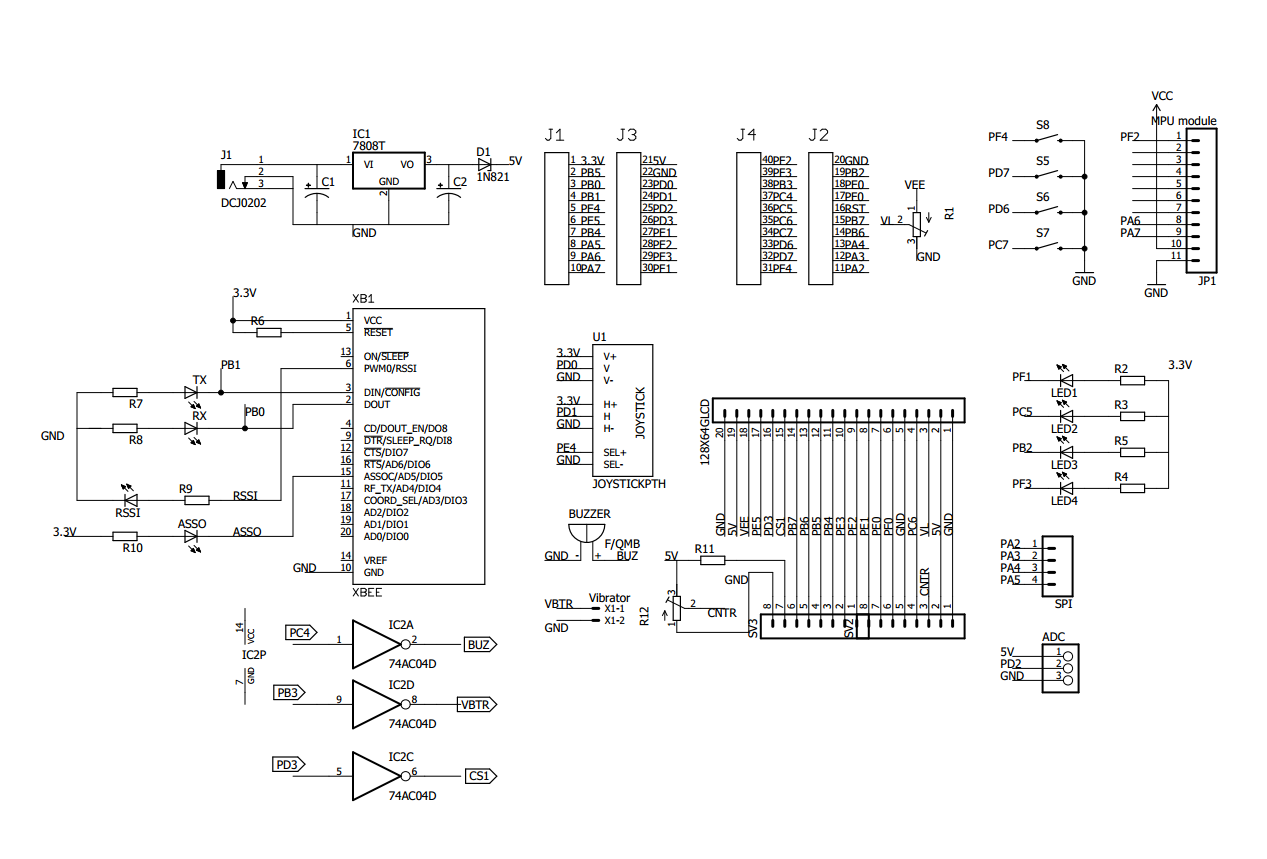
\includegraphics[width=15cm, height=10cm]{MiscImages/GAMECONSOLE_SCHEMATIC.png}
  \end{center}
  \item Links
  \begin{itemize}
  \item 
  \href{https://www.engineersgarage.com/sites/default/files/Graphics\%20LCD\%20JHD12864E\%20Datasheet.pdf}{GLCD Datasheet}
  \item
  \href{https://www.engineersgarage.com/sites/default/files/74LS04.pdf}{IC 7404 Datasheet}
  \end{itemize} 
\end{itemize}

\chapter{Software used}
\section{Code Composer Studio}
\qquad \textit{Code Composer Studio (CCStudio or CCS)} is an integrated development environment (IDE) to develop applications for Texas Instruments (TI) embedded processors. It has complete Windows, Linux and Mac\footnote[1]{Please note that only microcontroller and connectivity devices are supported on Mac. Processors devices are not supported.} support for the entire Texas Instruments portfolio, including the board used for the project, i.e., Tiva C TM4C123GH6PM Launchpad.
\subsection{Version Used}
\qquad Code Composer Studio Version:7.1.0.00016 is used throughout the project. Installation of RTOS, and training material are accessible directly through the Resource Explorer in this version.
\subsection{Downloading CCS}
Download the Windows installer from
\begin{enumerate}
\item \href{http://software-dl.ti.com/ccs/esd/CCSv7/CCS_7_1_0/exports/ccs_setup_7.1.0.00016.exe}{CCS(Windows) Web Installer} or
\item \href{http://software-dl.ti.com/ccs/esd/CCSv7/CCS_7_1_0/exports/CCS7.1.0.00016_win32.zip}{CCS(Windows) Offline Installer}. 
\end{enumerate} 
Download the macOS installer from
\begin{enumerate}
\item \href{http://software-dl.ti.com/ccs/esd/CCSv7/CCS_7_1_0/exports/CCS7.1.0.00016_web_osx.zip}{CCS(macOS) Web Installer} or
\item \href{http://software-dl.ti.com/ccs/esd/CCSv7/CCS_7_1_0/exports/CCS7.1.0.00016_osx.zip}{CCS(macOS) Offline Installer}. 
\end{enumerate} 
Linux versions can be installed from \href{http://processors.wiki.ti.com/index.php/Download_CCS}{CCS All Versions Download Page}. \\
\qquad The web installer will require Internet access until it completes. If the web installer version is unavailable or you can’t get it to work,download, unzip and run the offline version. The offline download will be much larger than the installed size of CCS since it includes all the possible supported hardware. 
\subsection{Installing CCS(Windows)}
Double click on the downloaded installer, after the installer has started, follow the steps mentioned below:\\
\begin{enumerate}
\item Accept the Software License Agreement and click Next.\\
{\begin{center}
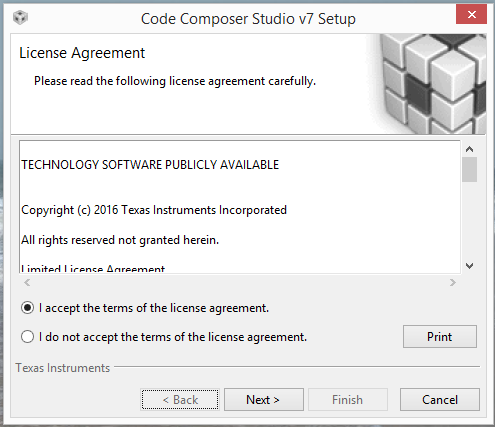
\includegraphics[width=6cm, height=6cm]{MiscImages/CCSInstall1}
\end{center}}
\item Select the destination folder and click next.\\
\begin{center}
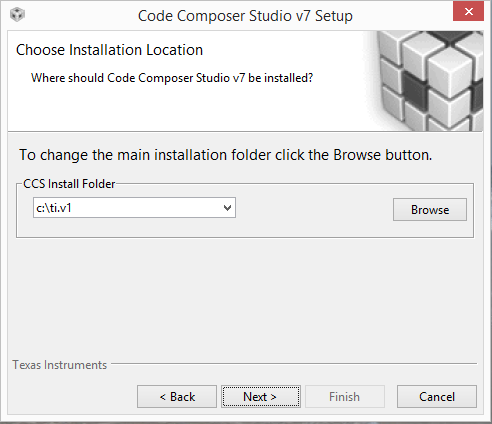
\includegraphics[width=6cm, height=6cm]{MiscImages/CCSInstall2}
\end{center}
\item Select the processors that your CCS installation will support. You must select "TM4C12X Arm Cortex M4". You can select other architectures, but the installation time and size will increase.\\
\begin{center}
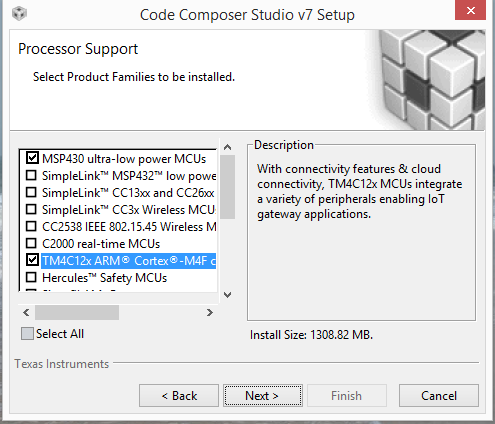
\includegraphics[width=6cm, height=6cm]{MiscImages/CCSInstall3}
\end{center}
\item Select debug probes and click finish \\
\begin{center}
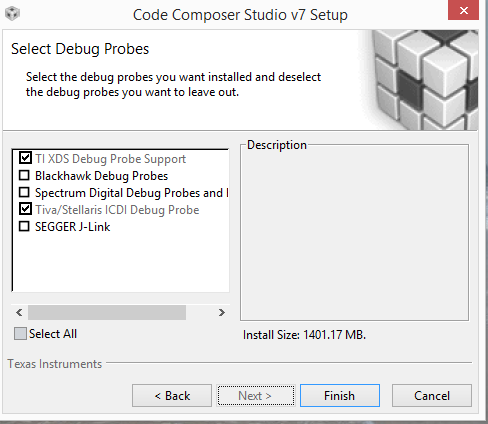
\includegraphics[width=6cm, height=6cm]{MiscImages/CCSInstall4}
\end{center}
\item The installer process	should take 15 - 30 minutes, depending on the speed of your connection. The offline installation should take 10 to 15 minutes. When the installation is complete, uncheck the “Launch Code Composer Studio v7” checkbox and then click Finish.There are several additional tools that require installation during the CCS install process. Click “Yes” or “OK” to proceed when these appear. \\
\item Download and install the latest full version of TivaWare from: \href{http://www.ti.com/tool/sw-tm4c}{Tivaware Install Link}. The installation is straightforward, and the driver library from Tivaware is used for development.
\end{enumerate}

\subsection{Installing CCS(macOS)}
Unzip the downloaded zip package, and double click on ccs\_setup\_xxx.app. The installer opens, and refer to steps 1-5 of Windows Installation, it is identical. \\
For Tivaware installation, download the .exe from \href{http://www.ti.com/tool/sw-tm4c}{Tivaware Install Link}, unzip using Unarchiver and copy the folder to the ti install location at /Applications/ti. Thus, Tivaware is set to be used on macOS.

\subsection{Installing TI-RTOS}

TI-RTOS can be installed directly from CCS App Center(recommended)
\begin{enumerate}
\item In the Search Box, search for RTOS.
\item Press Install.
\item Restart CCS.
\end{enumerate}
Additionally, RTOS can be directly downloaded and installed from the \href{http://software-dl.ti.com/dsps/dsps_public_sw/sdo_sb/targetcontent/tirtos/index.html}{TI-RTOS Download Page}, for the desired Operating System.
\\ \\
You can find additional information at these websites:\\
Launchpad Home page: \\ \href{http://www.ti.com/launchpad}{http://www.ti.com/launchpad}\\
Tiva C Series TM4C123G LaunchPad:\\ \href{http://www.ti.com/tool/ek-tm4c123gxl}{http://www.ti.com/tool/ek-tm4c123gxl} \\
TM4C123GH6PM Resources:\\ \href{http://www.ti.com/product/tm4c123gh6pm}{http://www.ti.com/product/tm4c123gh6pm} \\
LaunchPad Wiki:\\ \href{http://www.ti.com/launchpadwiki}{http://www.ti.com/launchpadwiki}

\section{Mikroelektronika GLCD Font Creator}
\qquad GLCD Font Creator enables the creation of personalized fonts, symbols and icons for LCDs and GLCDs. Create fonts and symbols from scratch, or by importing existing fonts on your system. It lets you modify and adjust them for your needs, apply effects and finally export them as source code for use in mikroC, mikroBasic or mikroPascal compilers.

\subsection{Downloading and Installing Mikroelektronika GLCD Font Creator}
Download the Windows Installer from their \href{https://download.mikroe.com/setups/additional-software/glcd-font-creator/glcd-font-creator-v120.zip}{official website}. The Install Wizard is pretty straightforward. \\
For macOS, download the same .exe. Then use Wine to open it(Tutorials on installing and using Wine on macOS can be found \href{https://www.davidbaumgold.com/tutorials/wine-mac/}{here}). 

\section{Hobbytronics BMP-LCD Converter}
\qquad This software converts a 2 colour BMP file into the hex character array that can be used in a program to display the graphic on the LCD screen. It can be downloaded from
\href{http://www.hobbytronics.co.uk/download/BMP-LCD.zip}{here}. It requires no installation.

\chapter{Software and Code}
Three software systems are implemented during the course of the project. They are:
\begin{enumerate}
\item Timed Bomb Controller
\item The Vending Machine Controller
\item The Breakout Game
\end{enumerate}

\section{Timed Bomb Controller}
\subsection{Problem Statement}
\qquad The time bomb has a control panel with an GLCD that shows the current value of the timeout and three buttons: UP, DOWN, and ARM. The user begins with setting up the time bomb using the UP and DOWN buttons to adjust the timeout in one-second steps. Once the desired timeout is selected, the user can arm the bomb by pressing the ARM button. When armed, the bomb starts decrementing the timeout every second and explodes when the timeout reaches zero. An additional safety feature is the option to defuse an armed bomb by entering a secret code. The secret defuse code is a certain combination of the UP,DOWN and LEFT buttons. Of course, the defuse code must be correctly entered before the bomb times out.
\subsection{StateChart Solution}
\begin{center}
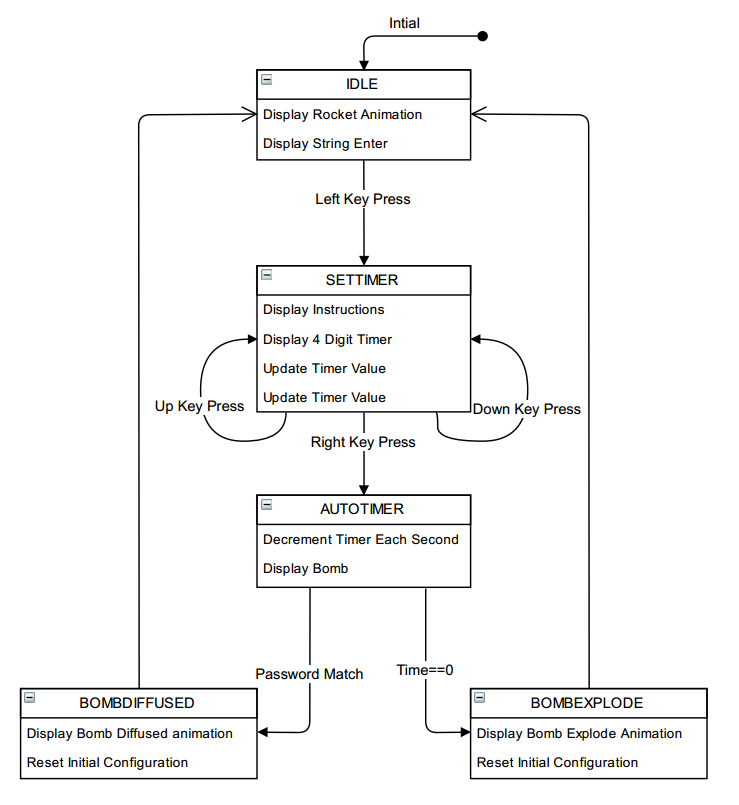
\includegraphics[width=10cm,height=10cm]{TimedBombImages/BombTimerStateChart}
\\{\small Fig a: TimerState Statechart} 
\end{center}
\qquad From the problem statement, the states of Timer Bomb over which its behaviour changes considerably are taken to be individual states of Timer Bomb.In this case, the Bomb Timer problem can be segregated into:
\begin{itemize}
  \item \textbf{{\small Idle}} State: \\ \qquad \qquad Perform basic initialization of 4 digit Timer, reset password and display animation.
    \begin{lstlisting}[basicstyle = \small, language = C]
        case idle:
          if(flag1 == 0)
          {
            // Display  once
              cal_time=120;
              glcd_frame1_write(); //Displays 
              // initial animation
              flag1=1;
          }
          break;
  \end{lstlisting}
  \item \textbf{{\small setTimer}} State: \\ \qquad \qquad Here UP and DOWN switches are used to set Timer. 4 Digit Timer is updated according to switch presses. MAX and MIN limits are 2 Minutes and 10 seconds respectively. RIGHT switch is used to arm bomb as illustrated in Fig a.
  \item \textbf{{\small autoTimer}} State: \\ \qquad \qquad In this state 4 Digit Timer starts decrementing till value reaches zero.  illustrated in Fig a.
      \begin{lstlisting}[basicstyle = \small, language = C]
  case autoTimer:
   // In autoTimer Mode, evaluate time and 
   // display the timer bits
      glcd_digit_write(bit_pos0,0);
      glcd_digit_write(bit_pos1,1);
      glcd_digit_write(bit_pos2,2);
      glcd_digit_write(bit_pos3,3);
      clear_section_glcd(2,0,78);
      glcd_bomb_write();
  // Switch to Bomb Explosion on Timeout
      if(cal_time==0)
      {
        flag5=1;
        flag4=0;
      }
  // Decrement Time
      if(cal_time>0)
      {
        cal_time--;
      }
      eval_time();
      break;
  \end{lstlisting}
  \item \textbf{{\small bombDiffused}} State: \\ \qquad \qquad No input from the user, but based on switch presses, the password is checked. Sequence is detected. If correct, Bomb is diffused. as illustrated in Fig a.
  \item \textbf{{\small bombExplode}} State: \\ \qquad \qquad No input from the user, but based on timer value. As Timer value reaches zero bomb Explodes. Animation for the same is displayed as illustrated in Fig a.
\end{itemize}
\subsection{Program Code}
\qquad The git repository for the complete code can be found \href{https://github.com/eYSIP-2017/eYSIP-2017_Game_Development-TI-RTOS/tree/master/Documentation/Timer\%20Bomb/Timer\%20Bomb\%20-\%20Code/TimedBomb_Final}{here}. It contains the complete project folder used in CCS. 
\begin{itemize}
  \item The console support libraries are present in the \href{https://github.com/eYSIP-2017/eYSIP-2017_Game_Development-TI-RTOS/tree/master/Documentation/Timer\%20Bomb/Timer\%20Bomb\%20-\%20Code/TimedBomb_Final/Console}{Console} folder. 
  \item timedbomb.c is the main file. This contains the Statechart and  the Timer Bomb abstraction.
\end{itemize}

\section{The Vending Machine Controller}
\subsection{Problem Statement}
\qquad The overall objective is to design a vending machine controller. The system has five digital inputs and three digital outputs. You can simulate the system with five switches and three LEDs. The inputs are \textit{quarter, dime, nickel, regular soda and diet soda} . The quarter input will go high, then go low when a 25\textcent \  coin is added to the machine. The dime and nickel inputs work in a similar manner for the 10\textcent \  and 5\textcent \ coins. The sodas cost 35\textcent \ each. The user presses the soda button to select a regular soda and the diet button to select a diet soda. The GiveSoda output will release a regular soda if pulsed high, then low. Similarly, the GiveDiet output will release a diet soda if pulsed high, then low. The Change output will release a 5\textcent \ coin if pulsed high, then low.
\subsection{Statechart Solution}
\begin{center}
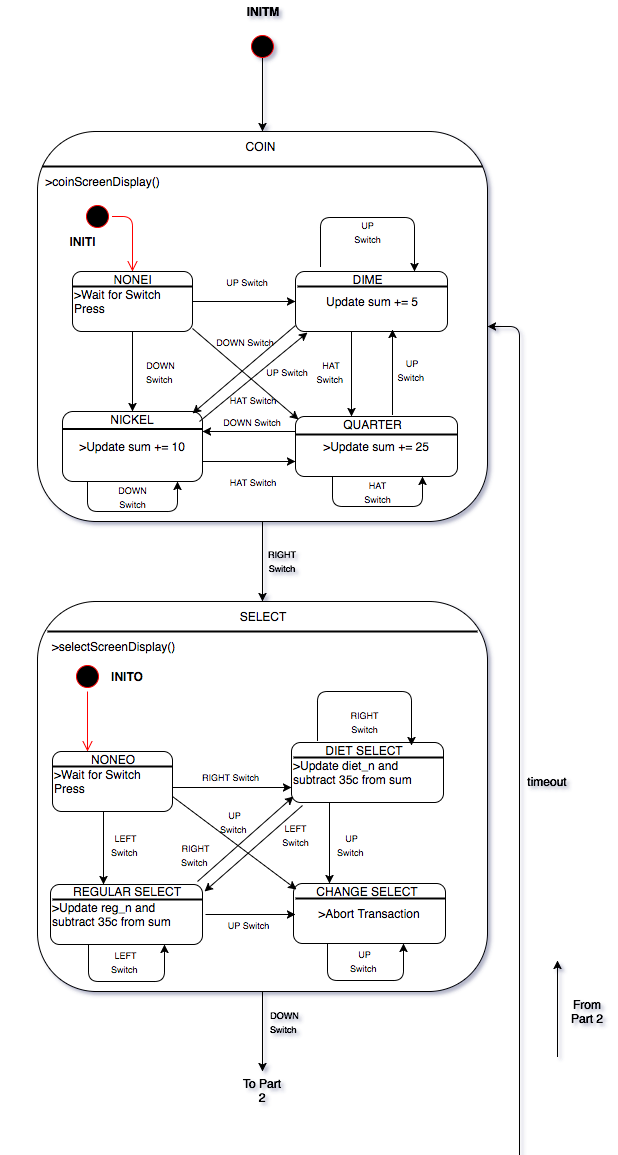
\includegraphics[width=10cm, height=18cm]{VendingMachineImages/VendingMachineStatechart1}
\\ {\small Fig a: Vending Machine Statechart Part 1}
\end{center}
\begin{center}
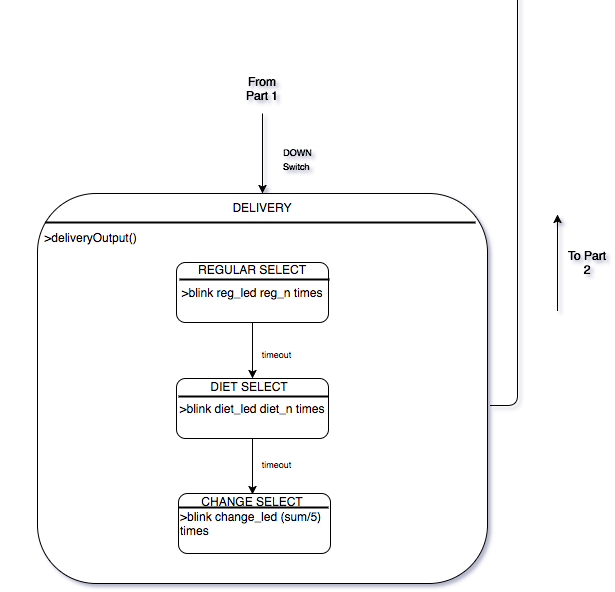
\includegraphics[width=10cm, height=9cm]{VendingMachineImages/VendingMachineStatechart2}
\\ {\small Fig b: Vending Machine Statechart Part 2}
\end{center}
\qquad From the problem statement, the states of vending machine over which its behaviour changes considerably are taken to be individual states of the vending machine. In this case, the vending machine problem can be segregated into:
\begin{itemize}
  \item \textbf{{\small INITM}} State: \\ \qquad \qquad Perform basic initialization of sum entered, number of regular and diet soda selected variables.
  \begin{lstlisting}[basicstyle = \small, language = C]
          case INITM:
            // Resets various variables.
            sum = 0;
            reg_n = 0;
            diet_n = 0;
            vm_mode = COIN;
            input = INITI; // for COIN state
            output = INITO; // for SELECT state
  \end{lstlisting}
  \item \textbf{{\small COIN}} State: \\ \qquad \qquad Switches correspond to coin entry, and coin entry GUI is displayed. (Unique Input and Output Behaviour). Internal transitions corresponding to each coin entry is as illustrated in Fig a.
  \item \textbf{{\small SELECT}} State: \\ \qquad \qquad Switches correspond to soda selection or cancel transaction, and Soda Selection GUI is displayed. It has internal state transitions corresponding to each selection as illustrated in Fig a.
  \item \textbf{{\small DELIVERY}} State: \\ \qquad \qquad No input from the user, but based on previous input, dispenses Regular Soda, Diet Soda and change through LED blinks and GLCD display. Internal transition between various states is as illustrated in Fig b.
\end{itemize}
\subsection{RTOS Implementation}
\qquad The use of statechart greatly simplifies task scheduling in RTOS. Here, basically two tasks are run as follows:
\begin{itemize}
  \item \textbf{{\small readInput()}} Task: \\ \qquad \qquad Handles switch press inputs. Has an internal state machine(implemented using the switch case construct) running as shown in the following code snippet:
  \begin{lstlisting}[basicstyle = \small, language = C]
        switch(vm_mode){
        case INITM:
            break;
        case COIN:
            coinScreenInput();
            break;
        case SELECT:
            selectScreenInput();
            break;
        case DELIVERY:
            // No user input in delivery state
            break;
        }
  \end{lstlisting}
  \item \textbf{{\small displayOutput()}} Task: \\ \qquad \qquad Handles GLCD display and LED blink outputs. Also has an internal state machine(implemented using the switch case construct) running as shown in the following code snippet:
  \begin{lstlisting}[basicstyle = \small, language = C]
        switch(vm_mode){
        case INITM:
            // Resets various variables.
            sum = 0;
            reg_n = 0;
            diet_n = 0;
            vm_mode = COIN;
            input = INITI;
            output = INITO;
        case COIN:
            coinScreenDisplay(); // Displays GUI for 
            break;               // coin entry state
        case SELECT:
            selectScreenDisplay(); // Displays GUI 
            break;          // for soda select state
        case DELIVERY:
            deliveryOutput(); // Handles Soda and 
            break;          // coin dispensing
        }
  \end{lstlisting}
\end{itemize}
\subsection{Program Code}
\qquad The git repository for the complete code can be found \href{https://github.com/eYSIP-2017/eYSIP-2017_Game_Development-TI-RTOS/tree/master/Documentation/Vending\%20Machine/Vending\%20Machine\%20-\%20Code/Implemented\%20Code}{here}. It contains the complete project folder used in CCS. 
\begin{itemize}
  \item The console support libraries are present in the \href{https://github.com/eYSIP-2017/eYSIP-2017_Game_Development-TI-RTOS/tree/master/Documentation/Vending\%20Machine/Vending\%20Machine\%20-\%20Code/Implemented\%20Code/Console}{Console} folder. 
  \item The font and graphic libraries are present in the \href{https://github.com/eYSIP-2017/eYSIP-2017_Game_Development-TI-RTOS/tree/master/Documentation/Vending\%20Machine/Vending\%20Machine\%20-\%20Code/Implemented\%20Code/Images}{Images} folder.
  \item VM\_RTOS.c is the main file. This contains the Statechart and RTOS implementation of the vending machine abstraction.
\end{itemize}
\section{The Breakout Game}
\subsection{Game Design}
\qquad The overall objective is to design the classic Breakout Game for the Tiva C Game Console, using the onboard peripherals.
The breakout game has a rectangular paddle at the bottom of the screen off which a moving ball ricochets off. At the top of the screen, it consists of rows of bricks. The victory condition is to clear the row of bricks, by hitting it with the ball. 
\begin{center}
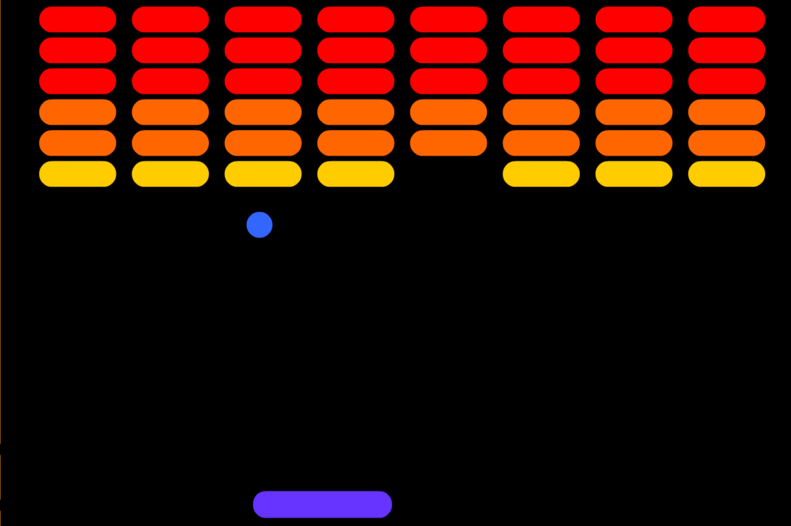
\includegraphics[width=10cm, height=8cm]{BreakoutImages/BreakoutDesign} \\
\caption{Fig 4.3(a): The Breakout Game Concept \\ Image Credits: \href{http://playsterr.com/wp-content/uploads/2016/01/breakout-voyager_img1.png}{Playsterr}} 
\end{center}
\\ Our implementation of the game is to have 5 types of bricks:
\begin{itemize}
  \item \textit{HARD} brick - Takes 3 hits to disappear.
  \item \textit{MEDIUM} brick - Takes 2 hits to disappear.
  \item \textit{EASY} brick - Takes 1 hit to disappear.
  \item \textit{MAGIC1} brick - Delivers a hit to all surrounding bricks.
  \item \textit{MAGIC2} brick - Increases paddle size for 10 seconds.
\end{itemize}
There are 3 difficulty levels:
\begin{itemize}
  \item \textit{EASY} - 3 lives, higher proportion of EASY bricks.
  \item \textit{MEDIUM} - 2 lives, higher proportion of MEDIUM bricks.
  \item \textit{HARD} - 1 life, higher proportion of HARD bricks.
\end{itemize}
Implicit above is an implementation of a life system(allowed number of retries for the player). There are three speeds for the ball:
\begin{itemize}
  \item \textit{SLOW} - Ball moves slowly.
  \item \textit{MEDIUM} - Ball moves at an average speed.
  \item \textit{FAST} - Ball moves very fast.
\end{itemize}
Additionally, the game has the following screens:
\begin{itemize}
  \item Entry Cutscene
  \item Menu Screen
  \item Instructions Screen(Accessible from the menu)
  \item Settings Screen(Accessible from the menu)
  \item Gameplay Screen
  \item Victory Screen
  \item Game Over Screen
\end{itemize}
\subsection{Statechart Solution}
\qquad Since the game has several active components at the same time, it runs several parallel state machines each of which may or may not be independent of the other. The different state machines are as follows:
\begin{center}
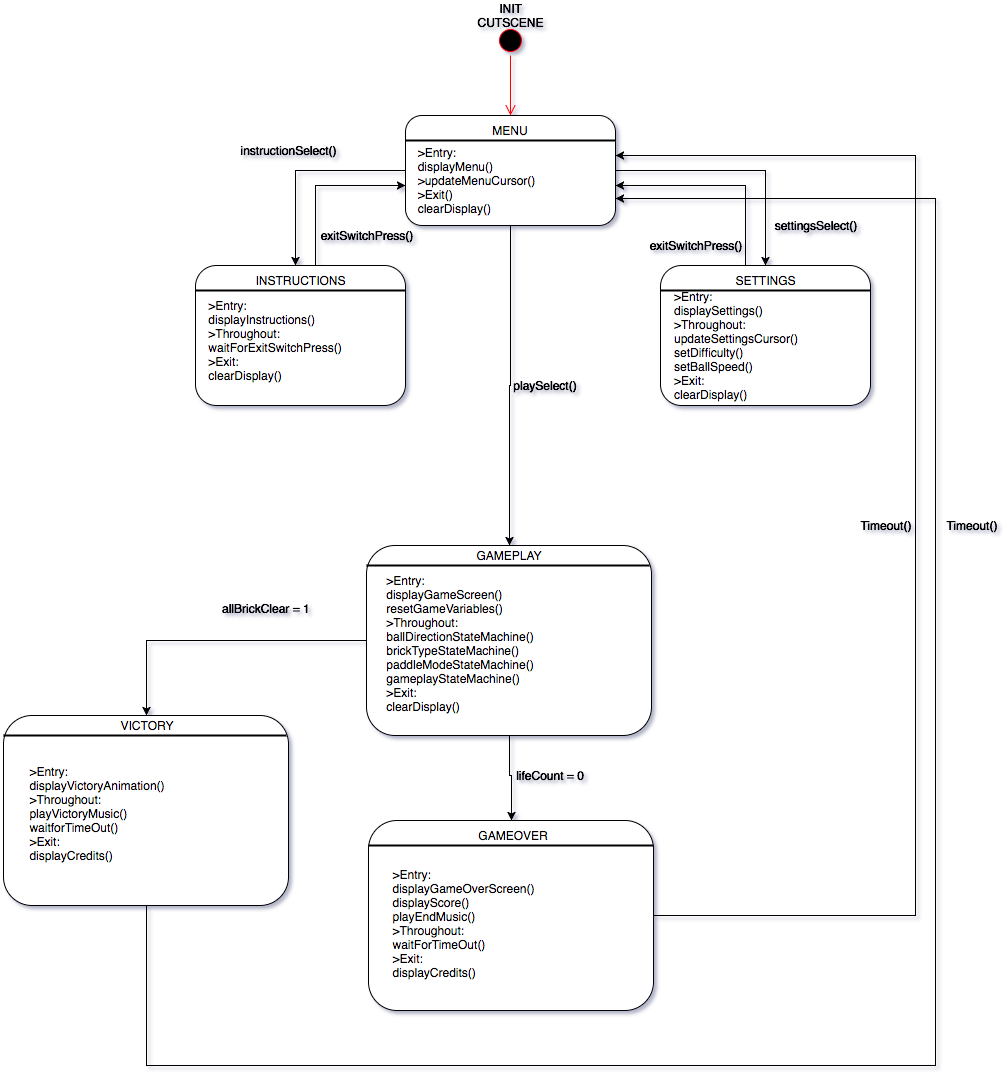
\includegraphics[width=14cm, height=18cm]{BreakoutImages/gameStateMachine} \\
\caption{Fig 4.3(b): Game Screens State Machine  \\
\end{center}
\newpage
\qquad The overall states in which the game exists is as shown in Fig 4.3(b). A brief explanation of each state is as follows:
\begin{itemize}
  \item \textbf{MENU} State: \\ \qquad This acts as the GUI for the user, and follows the initial cutscene(The Cutscene displays the cutscene graphic(as in Fig 5.3(a)) while playing Music).  The Menu Screen is as in Fig 5.3(b), and switch presses are used to move the cursor. 
  \\ \textit{RIGHT} Switch press is used for selection.
  \\ \textit{UP} Switch press is to move cursor up.
  \\ \textit{DOWN} Switch press is to move cursor down.
  \item \textbf{INSTRUCTIONS} State: \\ \qquad This displays instructions of gameplay for the user as in Fig. 5.3(c).
  \textit{LEFT} Switch Press = Back.
  \item \textbf{SETTINGS} State: \\ \qquad This allows for change of difficulty and ball speed settings for the player.
  \\ \textit{UP} Switch moves cursor up, and at topmost position, acts as back Switch.
  \\ \textit{DOWN} Switch moves cursor down, and at bottommost position, acts as back Switch.
  \\ \textit{LEFT} selects easiest setting, RIGHT selects toughest setting, HAT selects medium setting.
  \item \textbf{GAMEPLAY} State: \\ \qquad This is the actual gameplay screen running internal state machines. The gameplay screen is as in Fig 5.3(f).
  \\ Thumbstick moves paddle left or right.
  \item \textbf{GAME OVER} State: \\ \qquad Once the player runs out of lives, the game over screen is displayed which accepts no input(as in Fig 5.3(g)), but plays certain short music. Then returns to \textit{MENU} State.
  \item \textbf{VICTORY} State: \\ \qquad Once the player clears all bricks, a victory music is played over a victory screen(as in Fig 5.3h)), following end of music, game returns to \textit{MENU} State.
\end{itemize}
\begin{center}
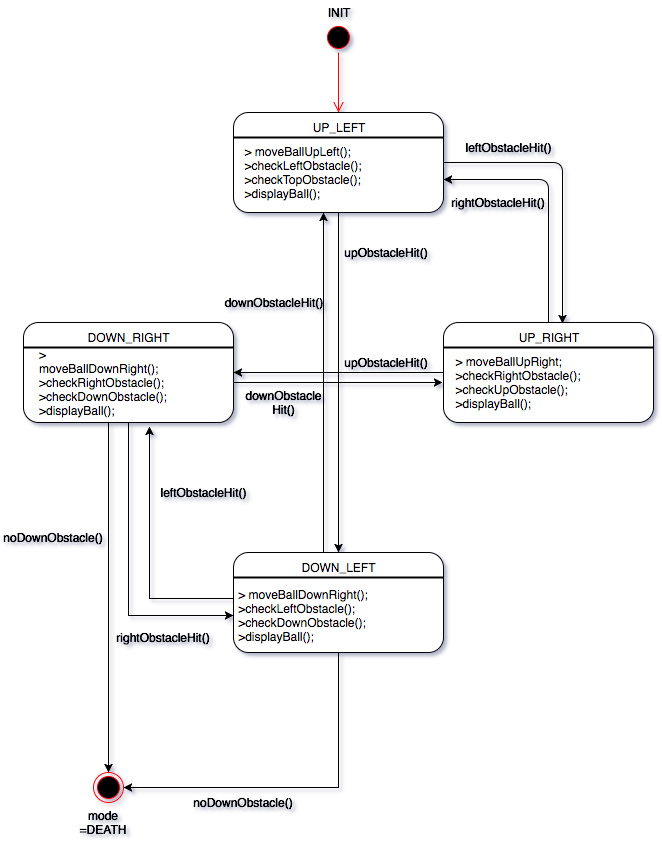
\includegraphics[width=14cm, height=16cm]{BreakoutImages/ballDirectionStatemachine} \\
\caption{Fig 4.3(c): Ball Direction State Machine} \\
\end{center}
\qquad Fig 4.3(c) shows the various modes of motion of the ball. Unless an obstacle is detected, the ball continues to be in a particular state. If the obstacle is a brick, \textit{hit} variable is decremented. If an obstacle is not present at the bottom, a life is lost.
\begin{center}
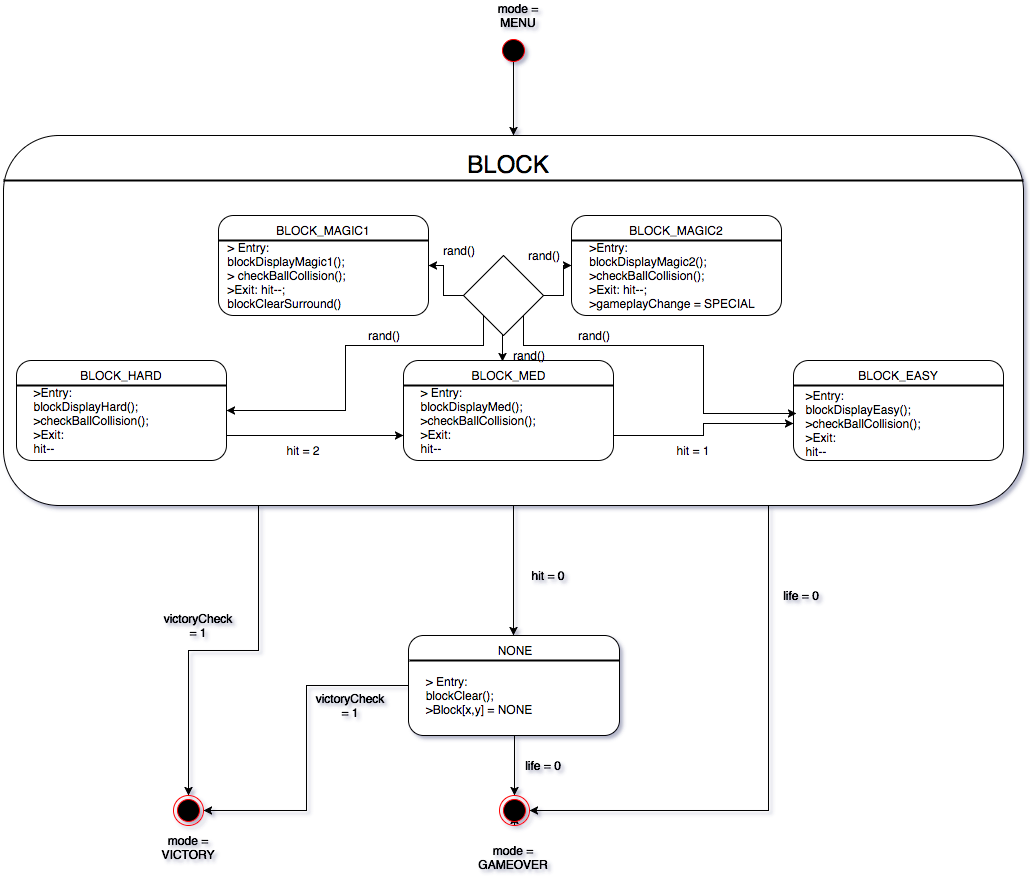
\includegraphics[width=14cm, height=14cm]{BreakoutImages/brickTypeStatemachine} \\
\caption{Fig 4.3(d): Brick Type State Machine} \\
\end{center}
\qquad The above state machine denotes switching between various states of each block. Initially, a randomizer randomizes the entire block wall. Thereafter, based on ball hit, different blocks are eliminated. The brick state machine is terminated upon \textit{DEATH} and \textit{VICTORY}.
\begin{center}
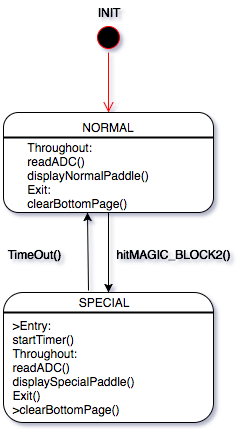
\includegraphics[width=4cm, height=7cm]{BreakoutImages/paddleTypeStateMachine} \\
\caption{Fig 4.3(e): Paddle Type State Machine} \\
\end{center}
\qquad The visualization above represents the two different states for the paddle, the special extended state for 10 seconds once the ball hits BLOCK\_MAGIC2 and the normal state otherwise. Each state reads from ADC and displays the paddle at the appropriate position.
\begin{center}
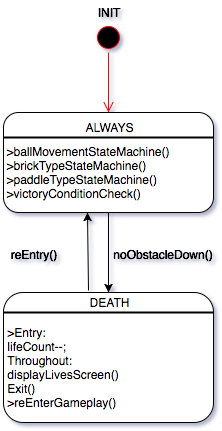
\includegraphics[width=4cm, height=7cm]{BreakoutImages/gameplayStateMachine}\\
\caption{Fig 4.3(f): Gameplay Internal State Machine} \\
\end{center}
\qquad The above state machine shows two different states within gameplay. Gameplay continues till the player dies, upon which, certain tasks are performed as illustrated in Fig 4.3(f) above.
\subsection{RTOS Implementation}
\qquad RTOS is absolutely necessary to maintain seamless execution of several different simultaneous gameplay components. Here, basically two tasks are run as follows:
\begin{itemize}
  \item \textbf{{\small readInput()}} Task: \\ \qquad \qquad Handles switch press and ADC inputs. Has an internal state machine(implemented using the switch case construct) running.
  \item \textbf{{\small displayOutput()}} Task: \\ \qquad \qquad Handles GLCD display, LED blink, motor vibration and Buzzer outputs. Also has an internal state machine(implemented using the switch case construct) running.
\end{itemize}
\subsection{Program Code}
\qquad The git repository for the complete code can be found \href{https://github.com/eYSIP-2017/eYSIP-2017_Game_Development-TI-RTOS/tree/master/Documentation/Breakout/Breakout\%20-\%20Code/Implemented\%20Code}{here}. It contains the complete project folder used in CCS. 
\begin{itemize}
  \item The console support libraries(including the font libraries) are present in the \href{https://github.com/eYSIP-2017/eYSIP-2017_Game_Development-TI-RTOS/tree/master/Documentation/Breakout/Breakout\%20-\%20Code/Implemented\%20Code/Console}{Console} folder. 
  \item The game objects are present in the \href{https://github.com/eYSIP-2017/eYSIP-2017_Game_Development-TI-RTOS/tree/master/Documentation/Breakout/Breakout\%20-\%20Code/Implemented\%20Code/Objects}{Objects} folder.
    \item The game screens are present in the \href{https://github.com/eYSIP-2017/eYSIP-2017_Game_Development-TI-RTOS/tree/master/Documentation/Breakout/Breakout\%20-\%20Code/Implemented\%20Code/Screens}{Screens} folder.
  \item game.c is the main file. This contains the two basic tasks part of RTOS, with their internal state machines. Additional functions are used from above libraries.
\end{itemize}
\chapter{Use and Demo}
\section{Timer Bomb - Images}
\begin{center}

\includegraphics[width=10cm, height=5cm]{TimedBombImages/enterScreen} \\
\\ {\small Fig 5.1(a): Initial} \\
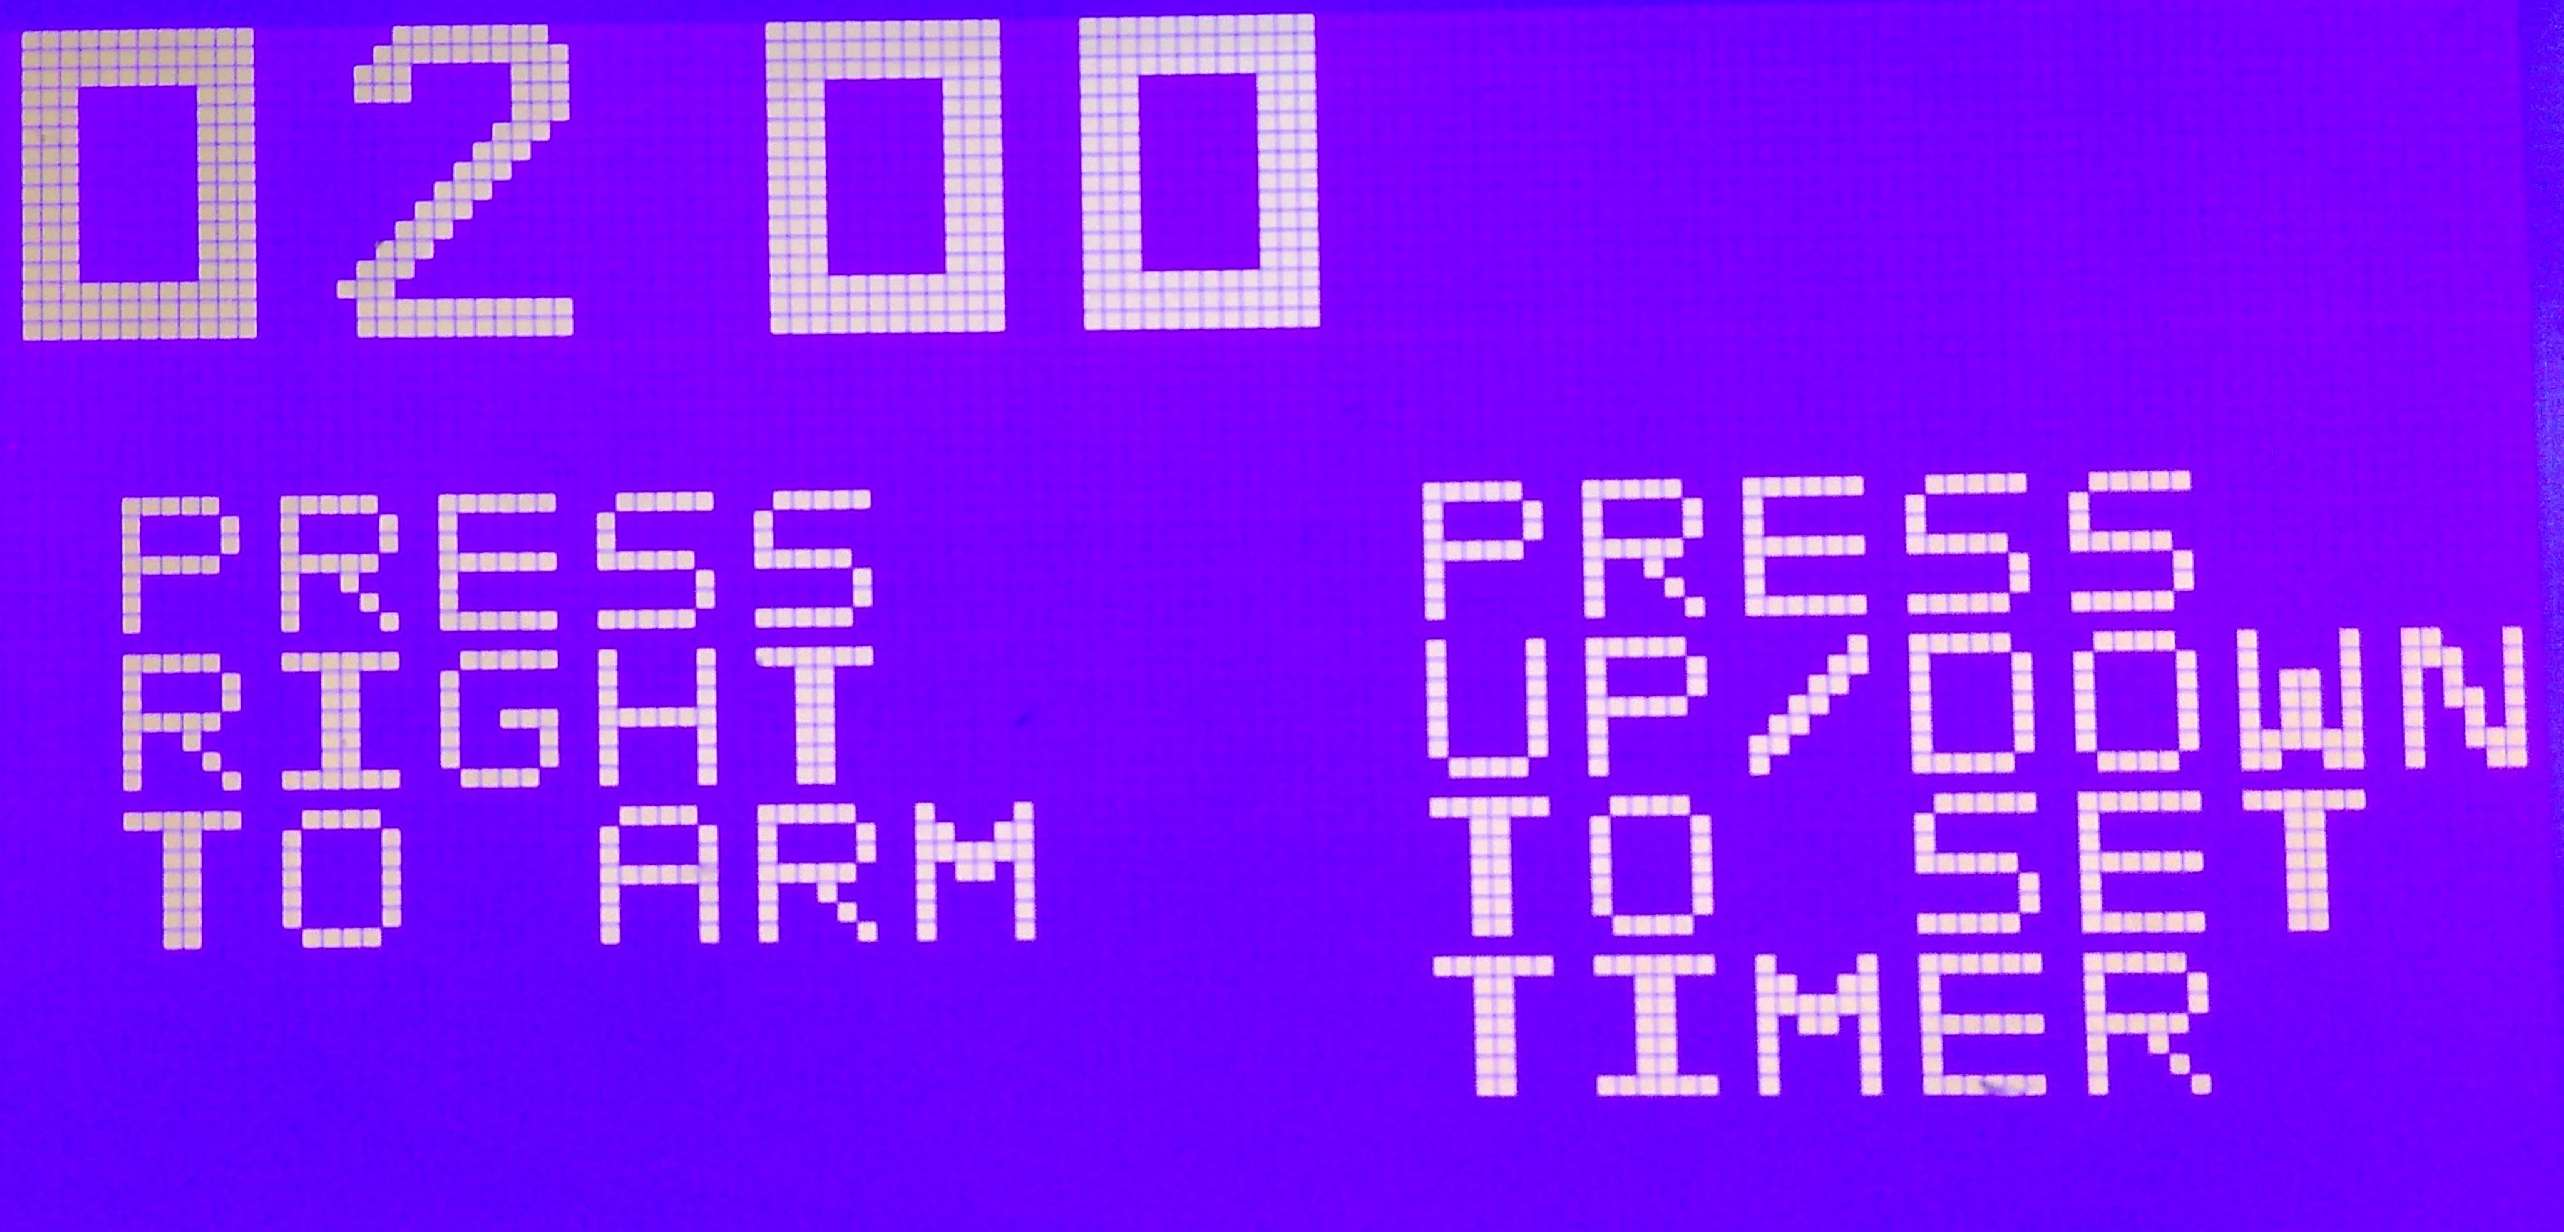
\includegraphics[width=10cm, height=5cm]{TimedBombImages/setTimerScreen} \\
\\ {\small Fig 5.1(b): Set the timer} \\
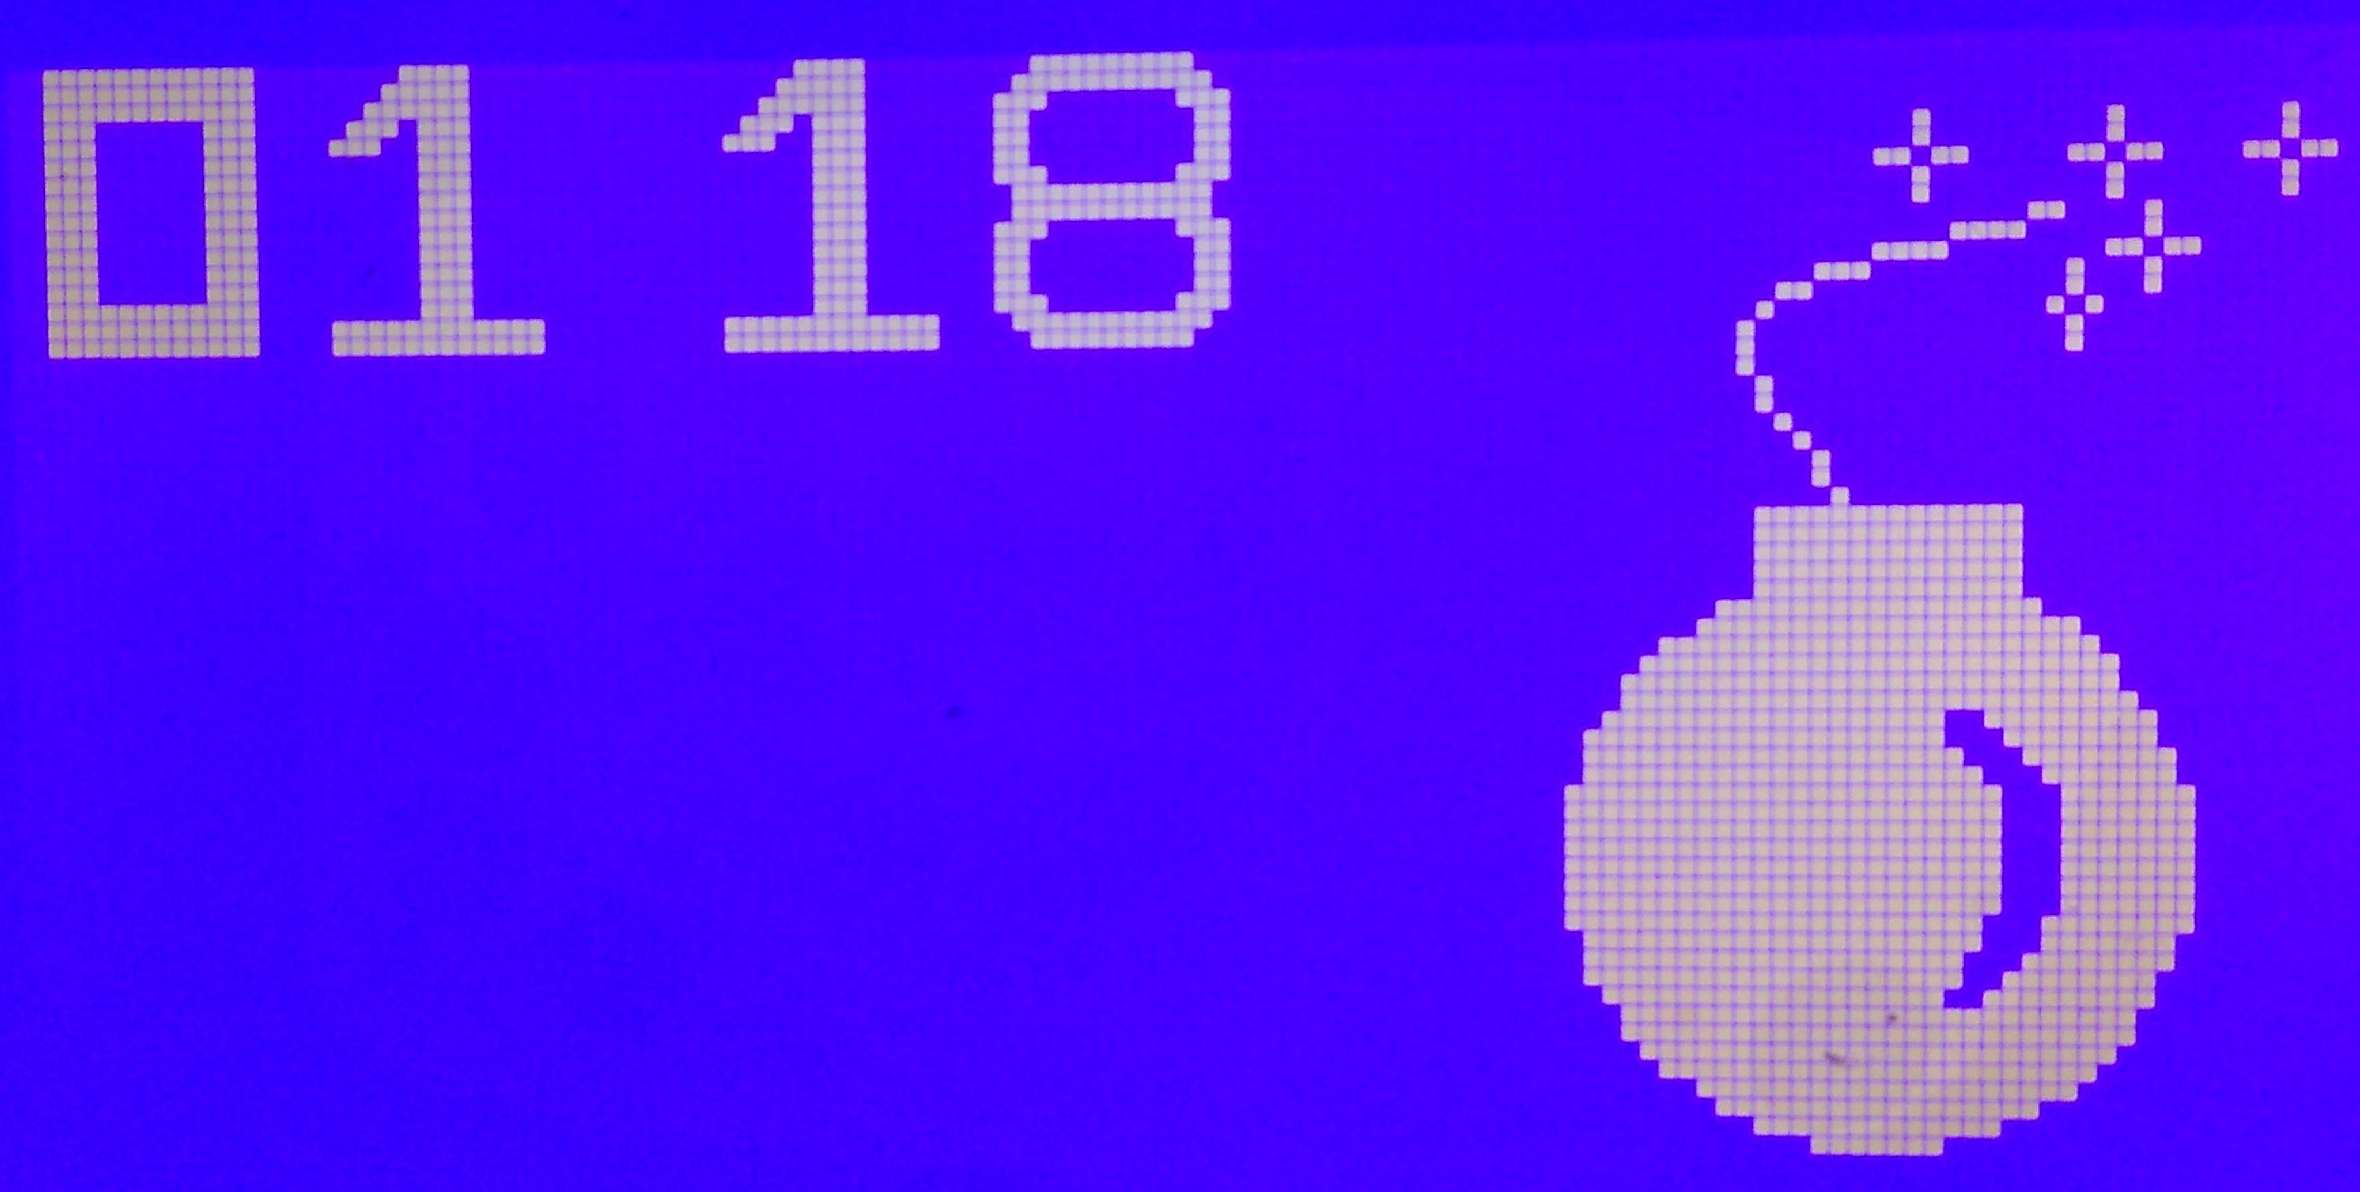
\includegraphics[width=10cm, height=5cm]{TimedBombImages/countdownTimer} \\
\\ {\small Fig 5.1(c): Timer Counting Down} \\
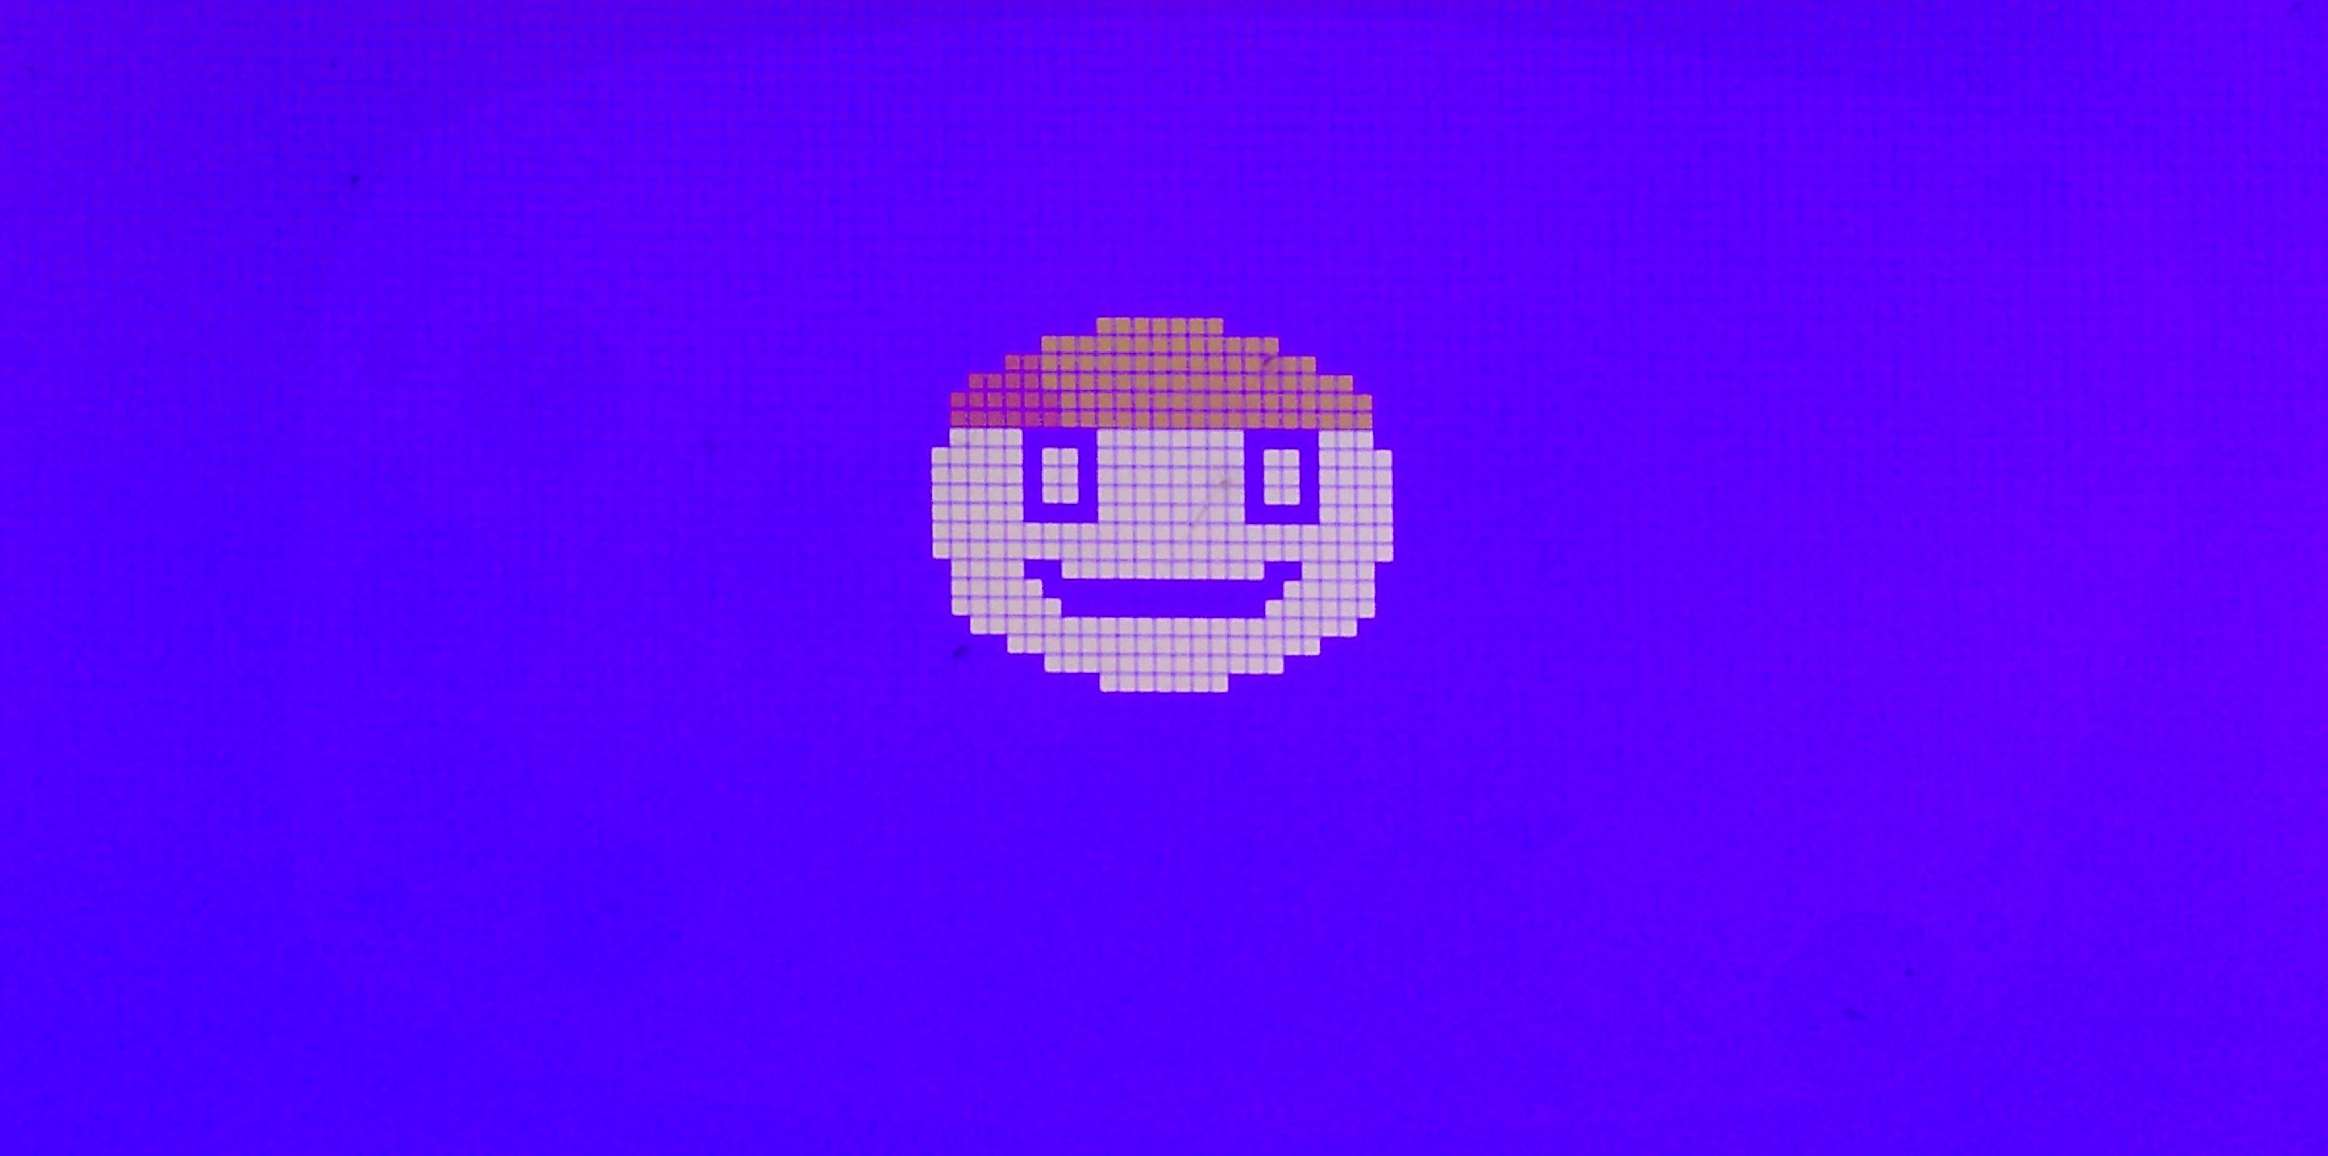
\includegraphics[width=10cm, height=5cm]{TimedBombImages/bombDiffusedScreen} \\
\\ {\small Fig 5.1(d): Successfully Diffused Screen} \\

\includegraphics[width=10cm, height=5cm]{TimedBombImages/deathScreen} \\
\\ {\small Fig 5.1(e): Death after Bomb Explosion} \\
\end{center}
\section{Vending Machine - Images}
\begin{center}
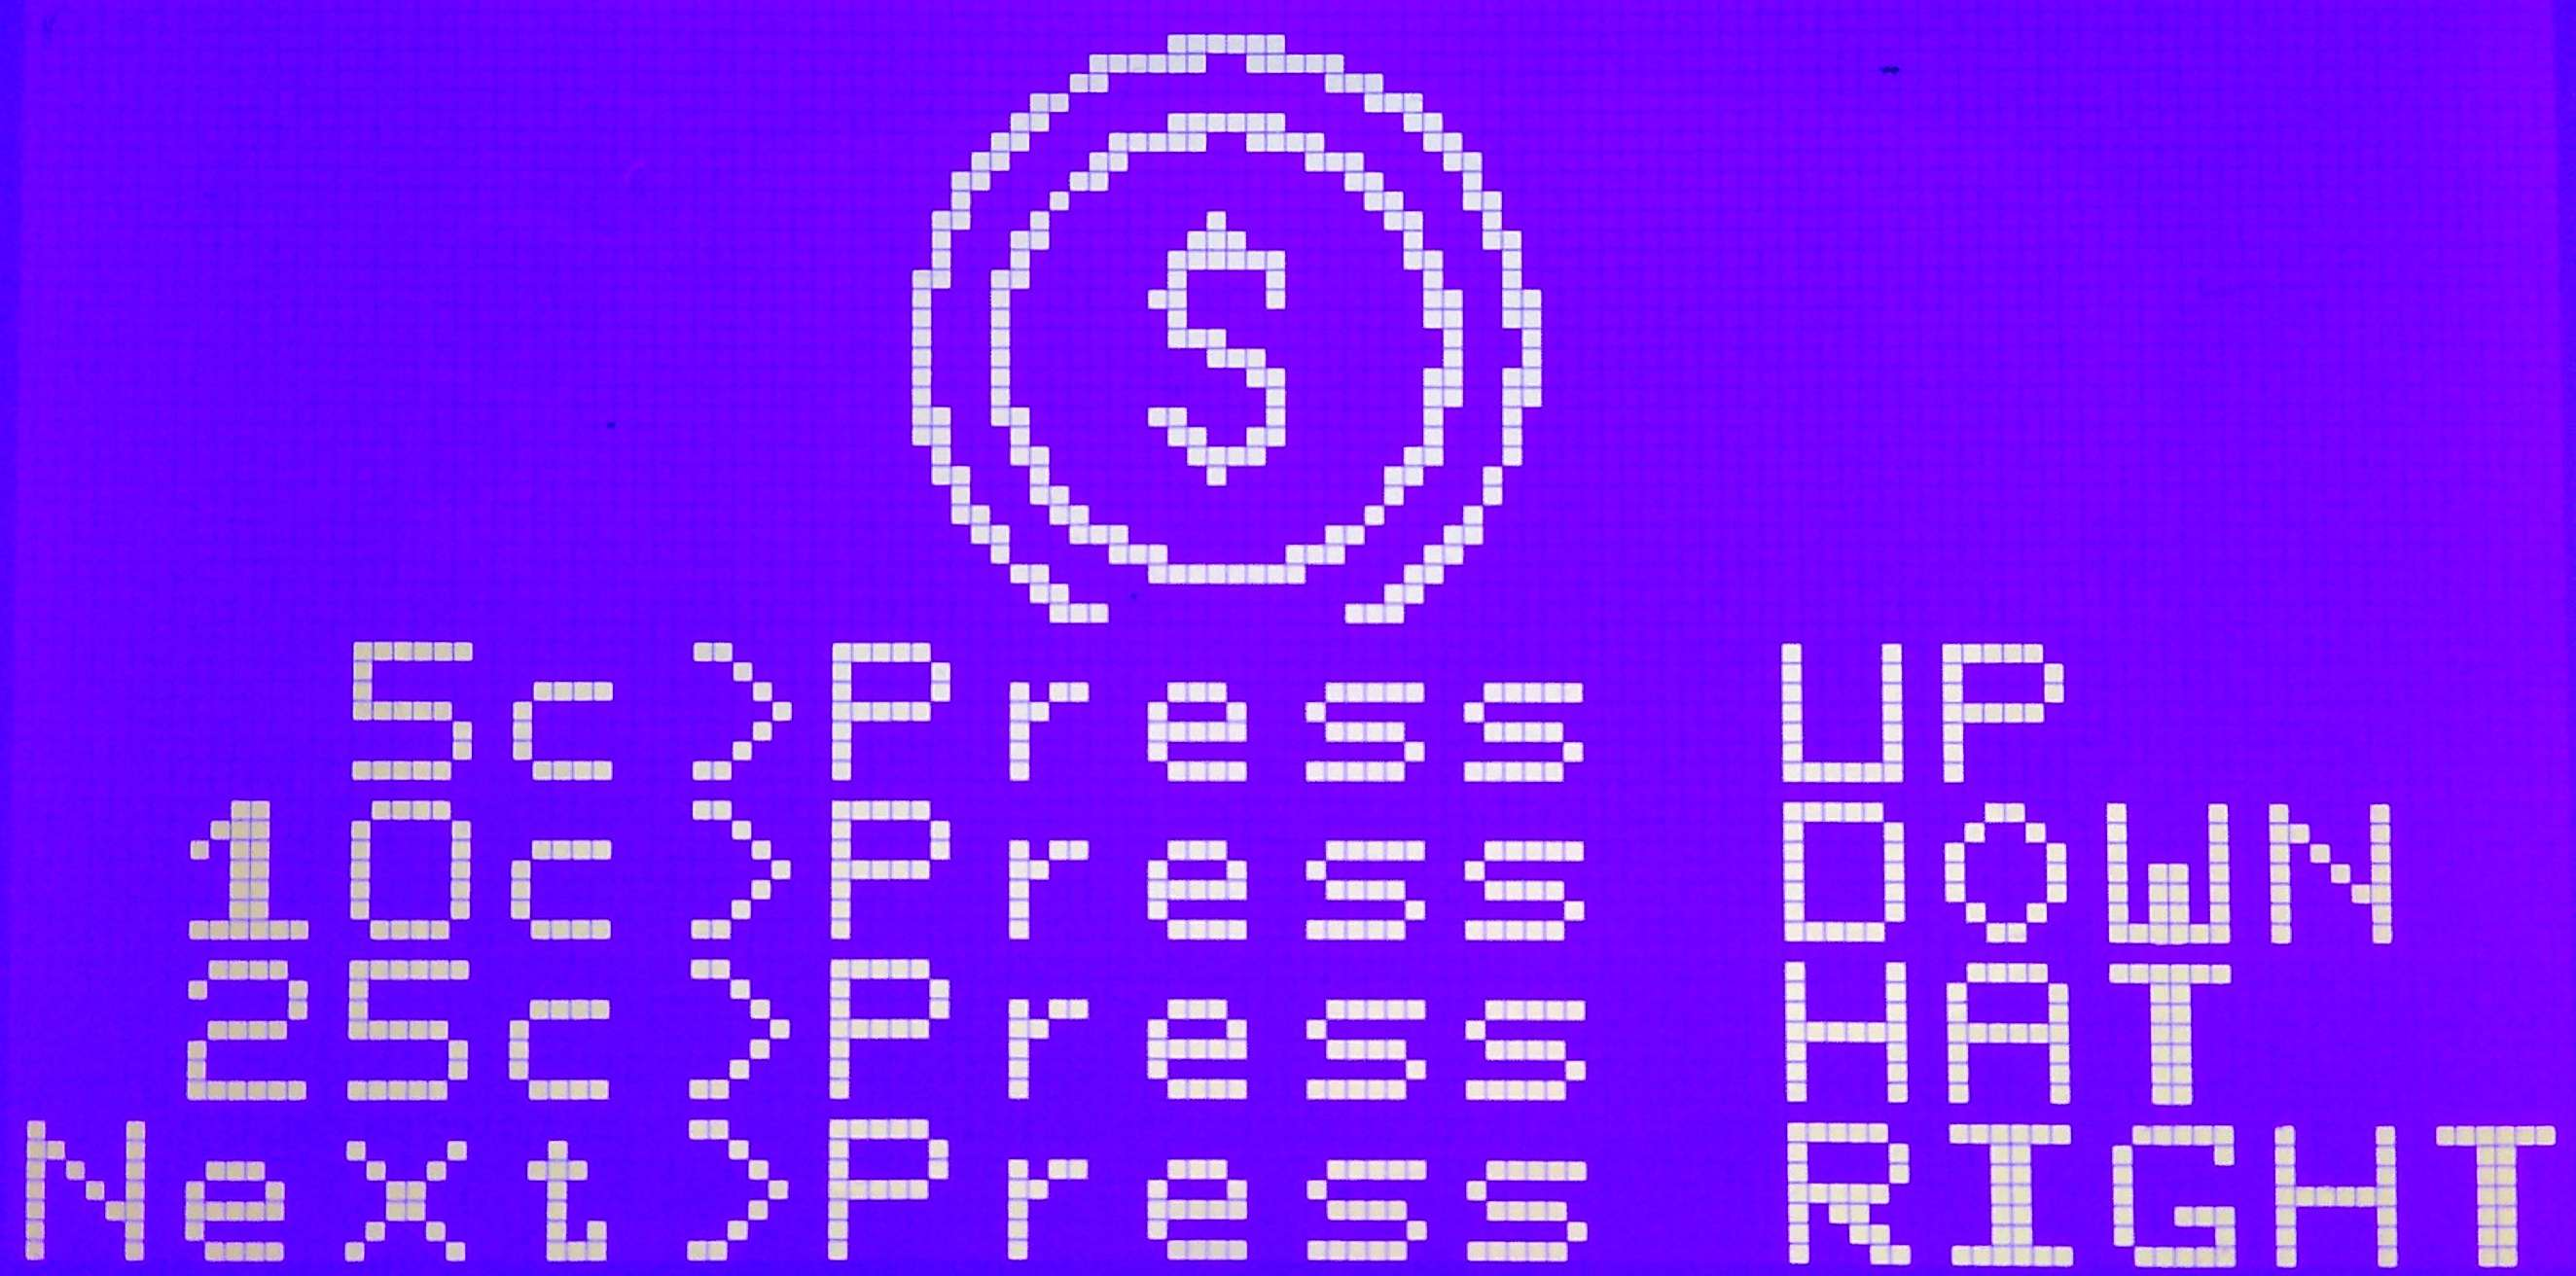
\includegraphics[width=10cm, height=5cm]{VendingMachineImages/COIN} \\
{\small Fig 5.2(a): Coin Entry Screen} \\
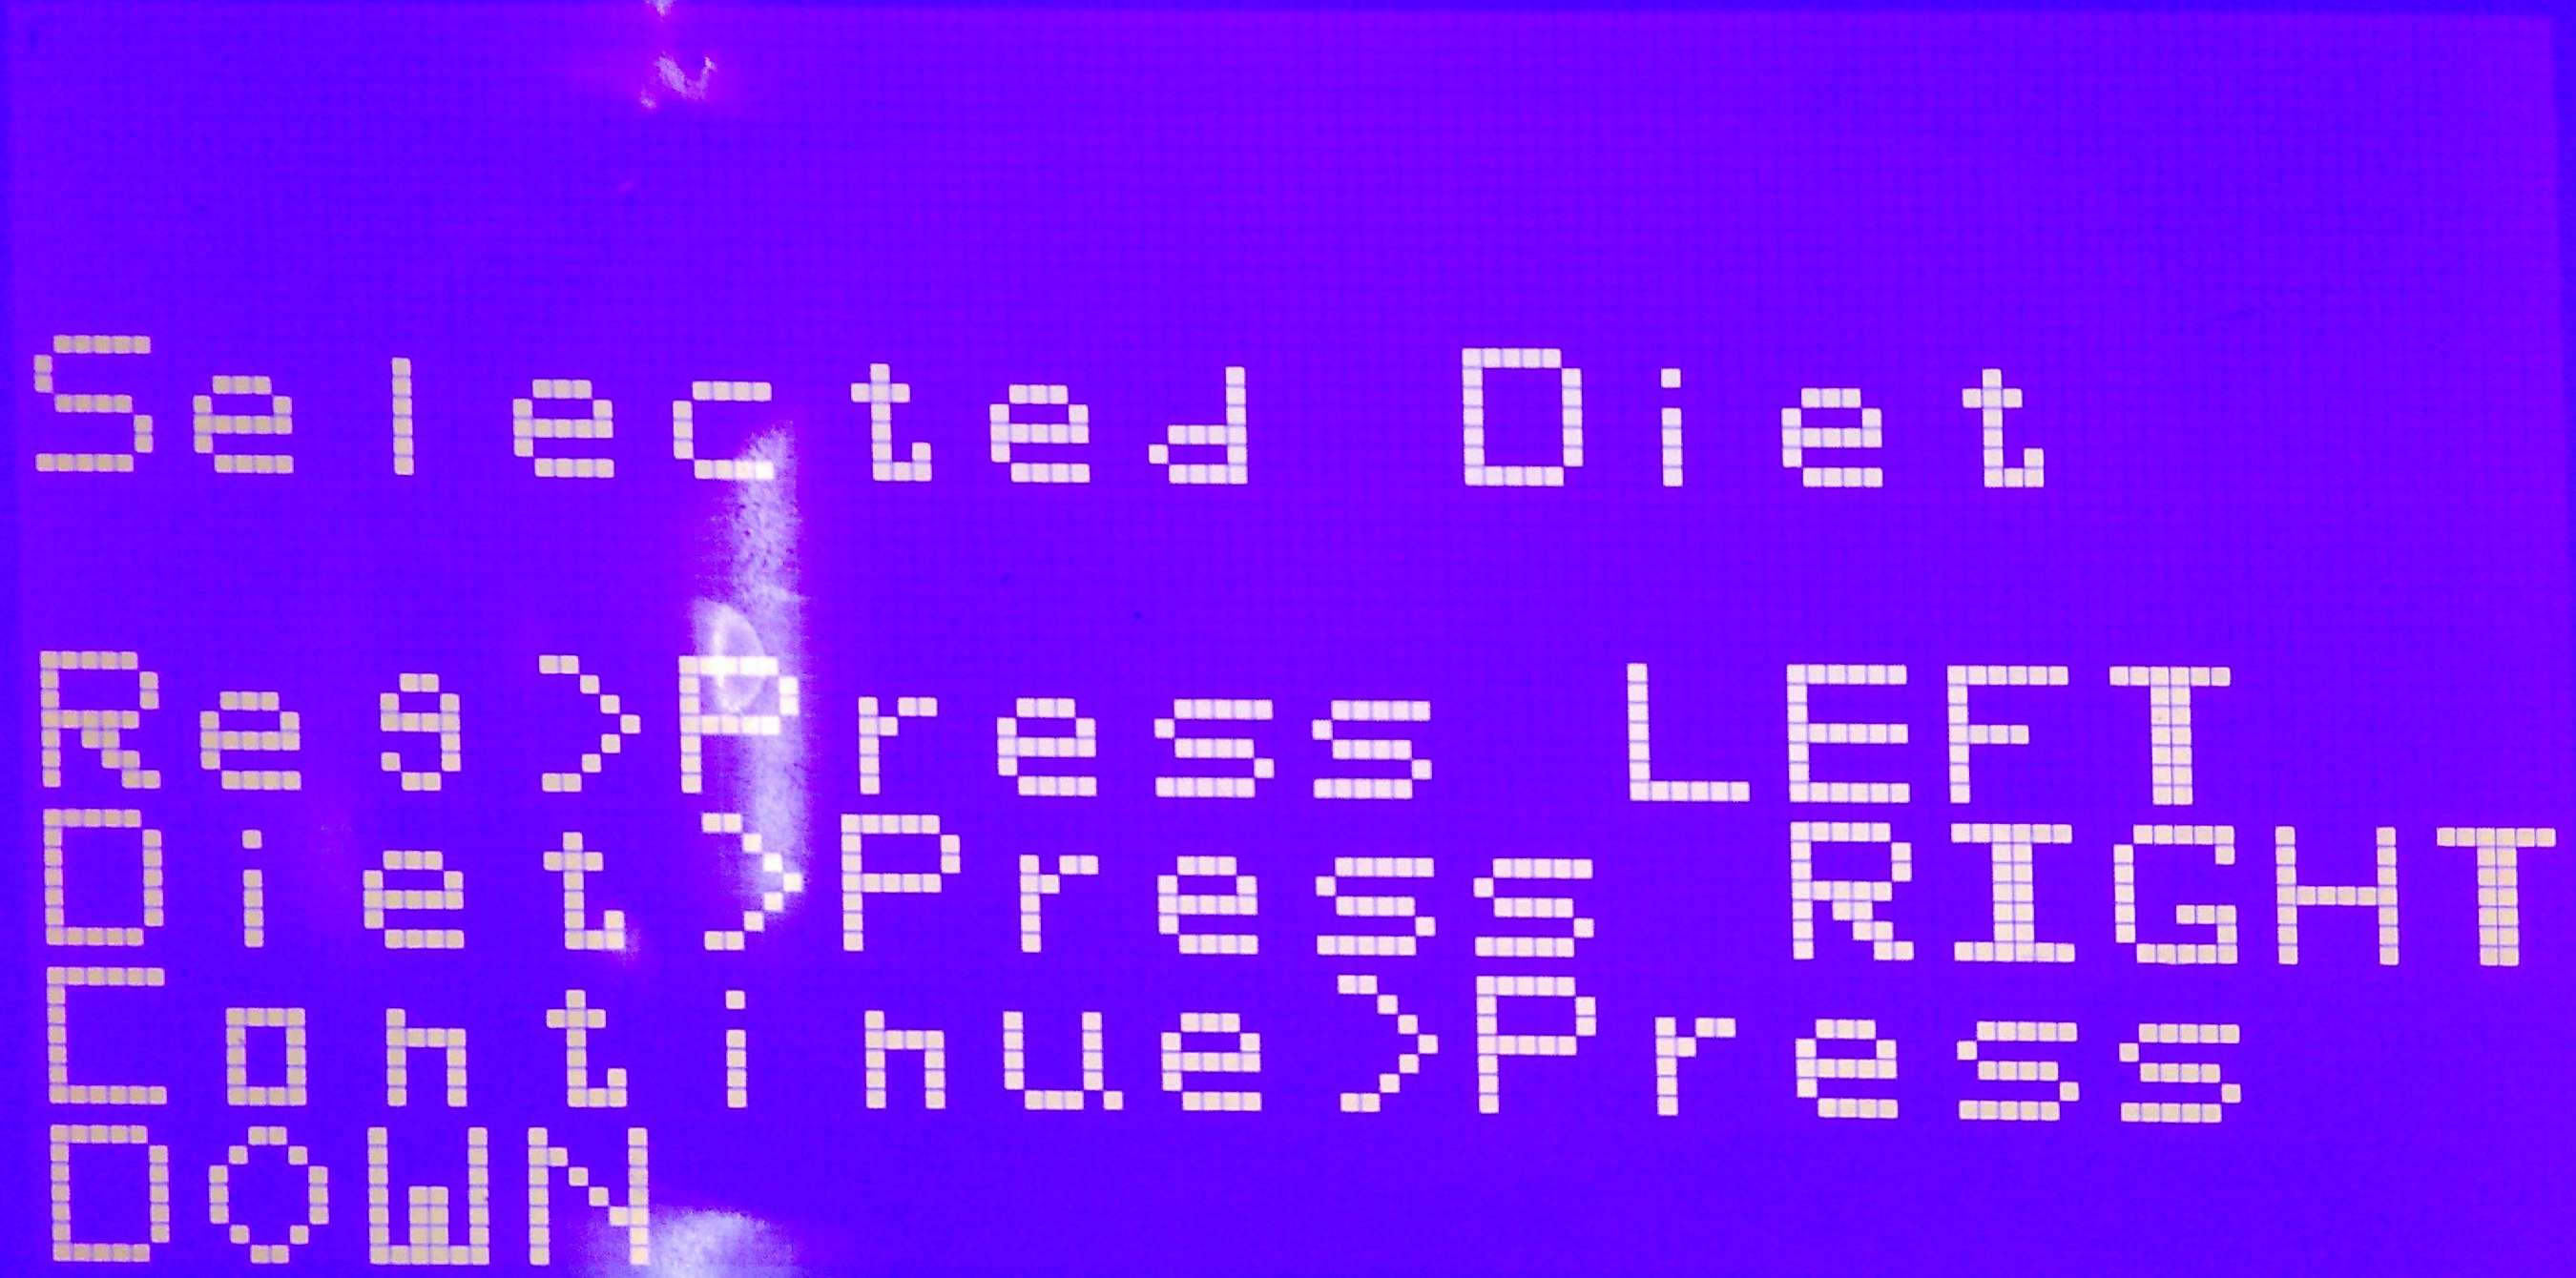
\includegraphics[width=10cm, height=5cm]{VendingMachineImages/SODASELECT} \\
{\small Fig 5.2(b): Soda Selection Screen} \\
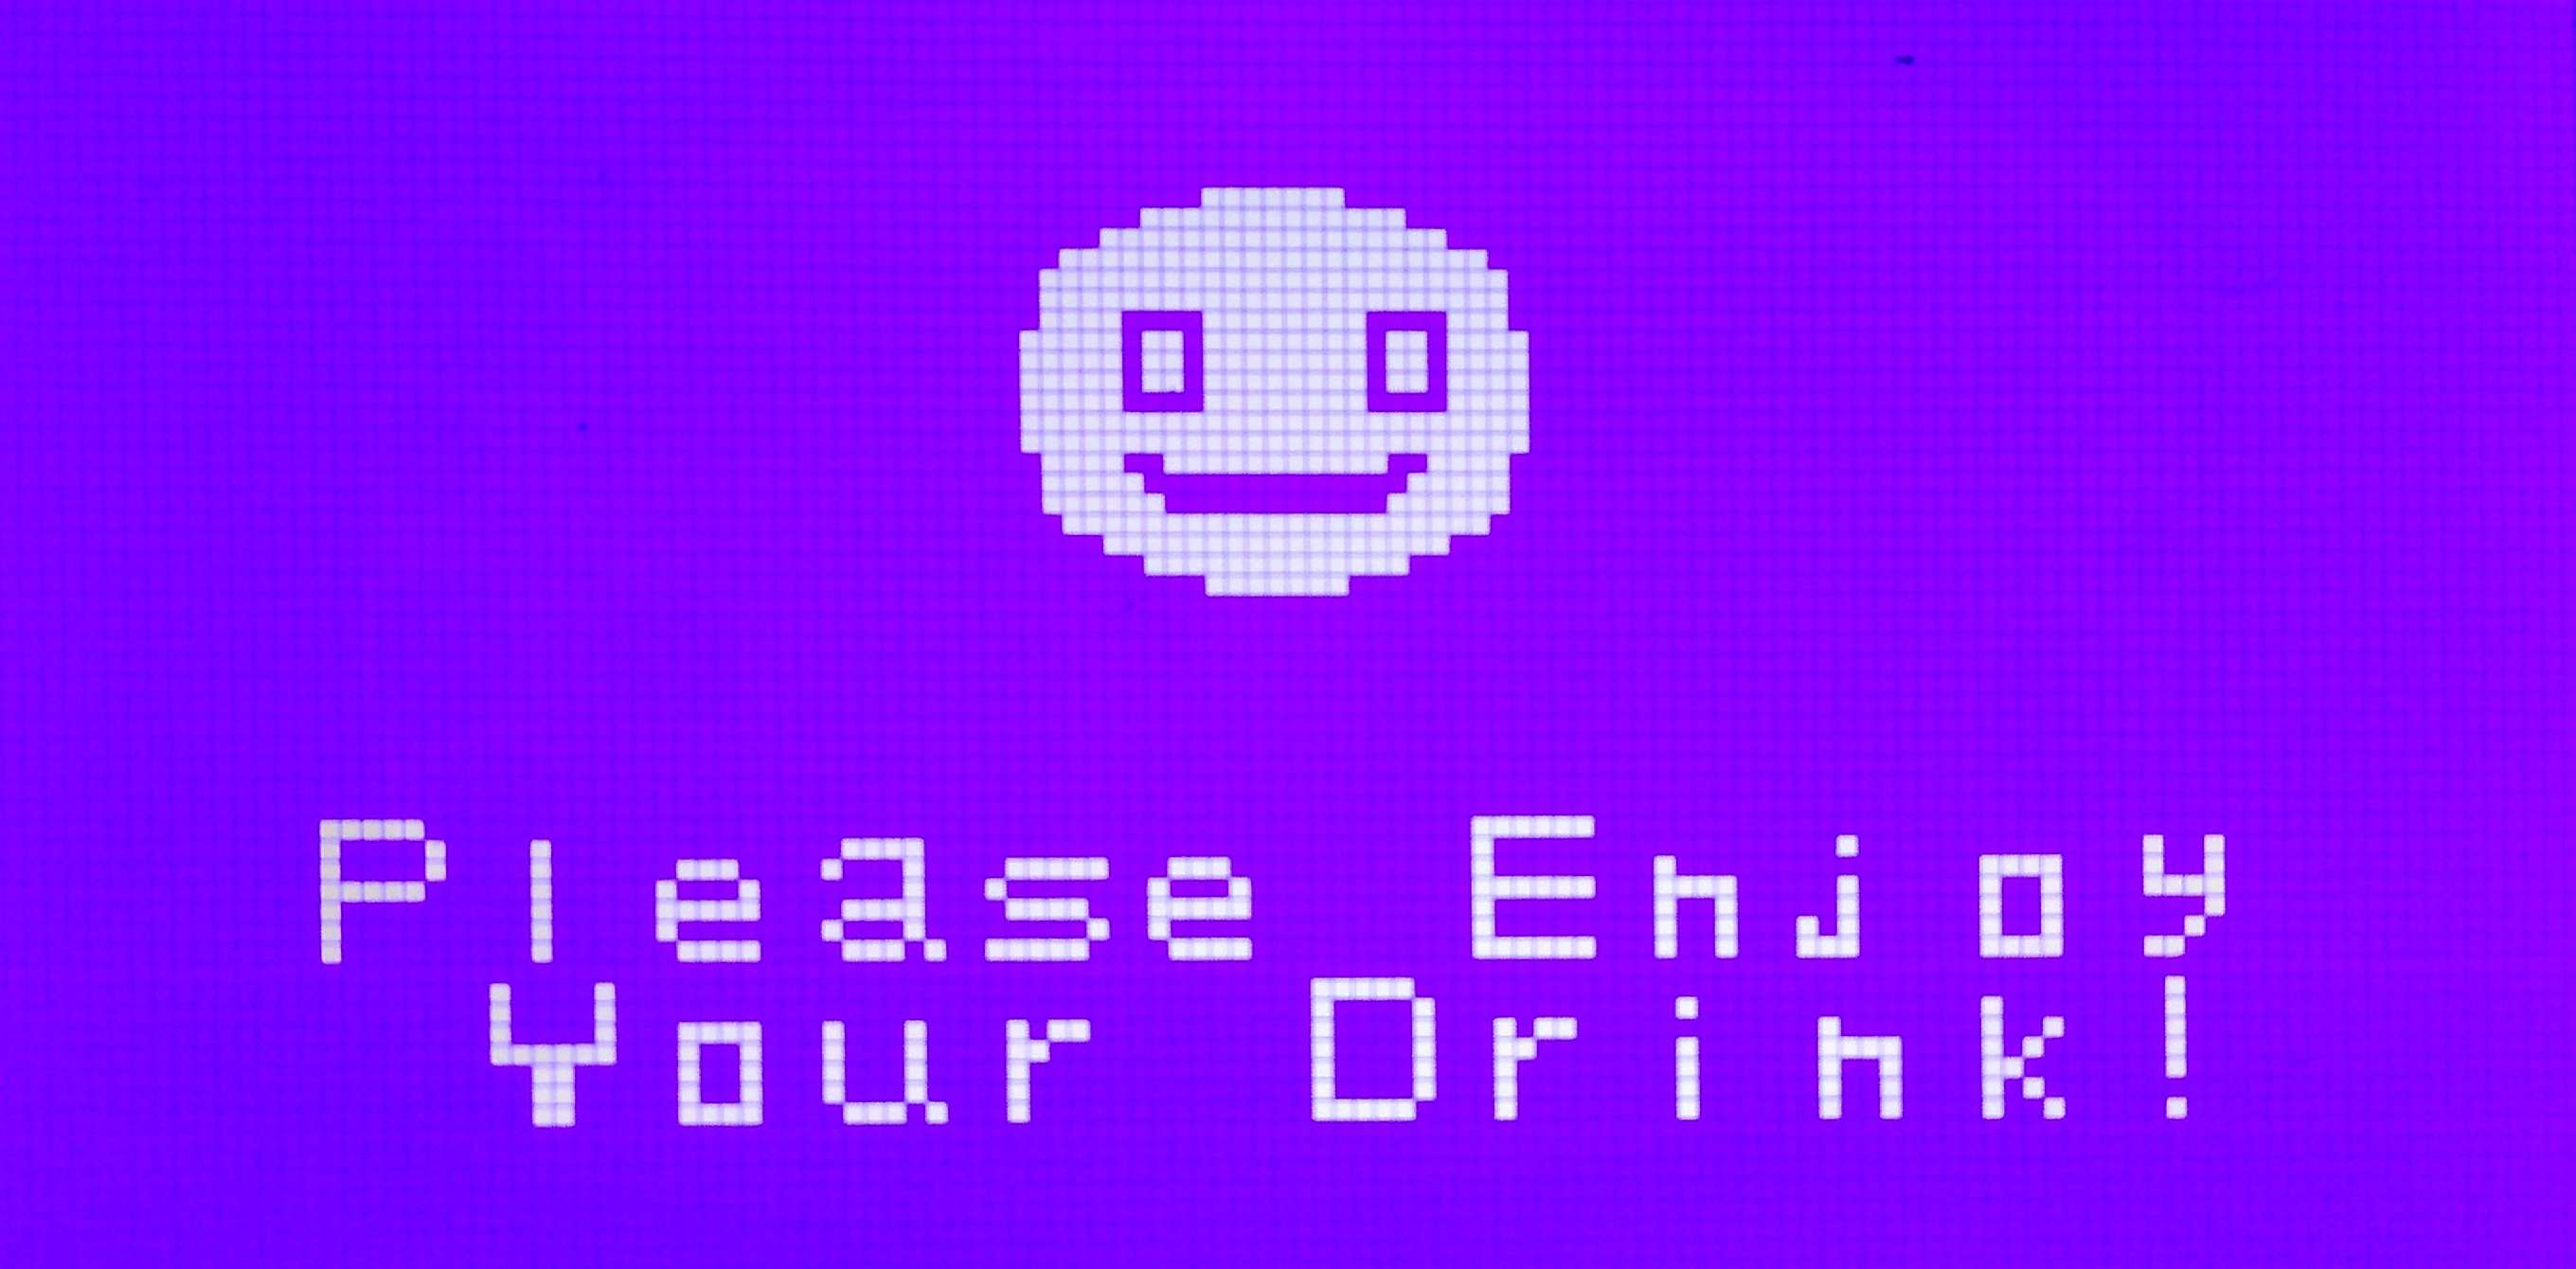
\includegraphics[width=10cm, height=5cm]{VendingMachineImages/DELIVERY} \\
{\small Fig 5.2(c): Delivery Screen} \\
\end{center}
\section{The Breakout Game - Images}
\begin{center}
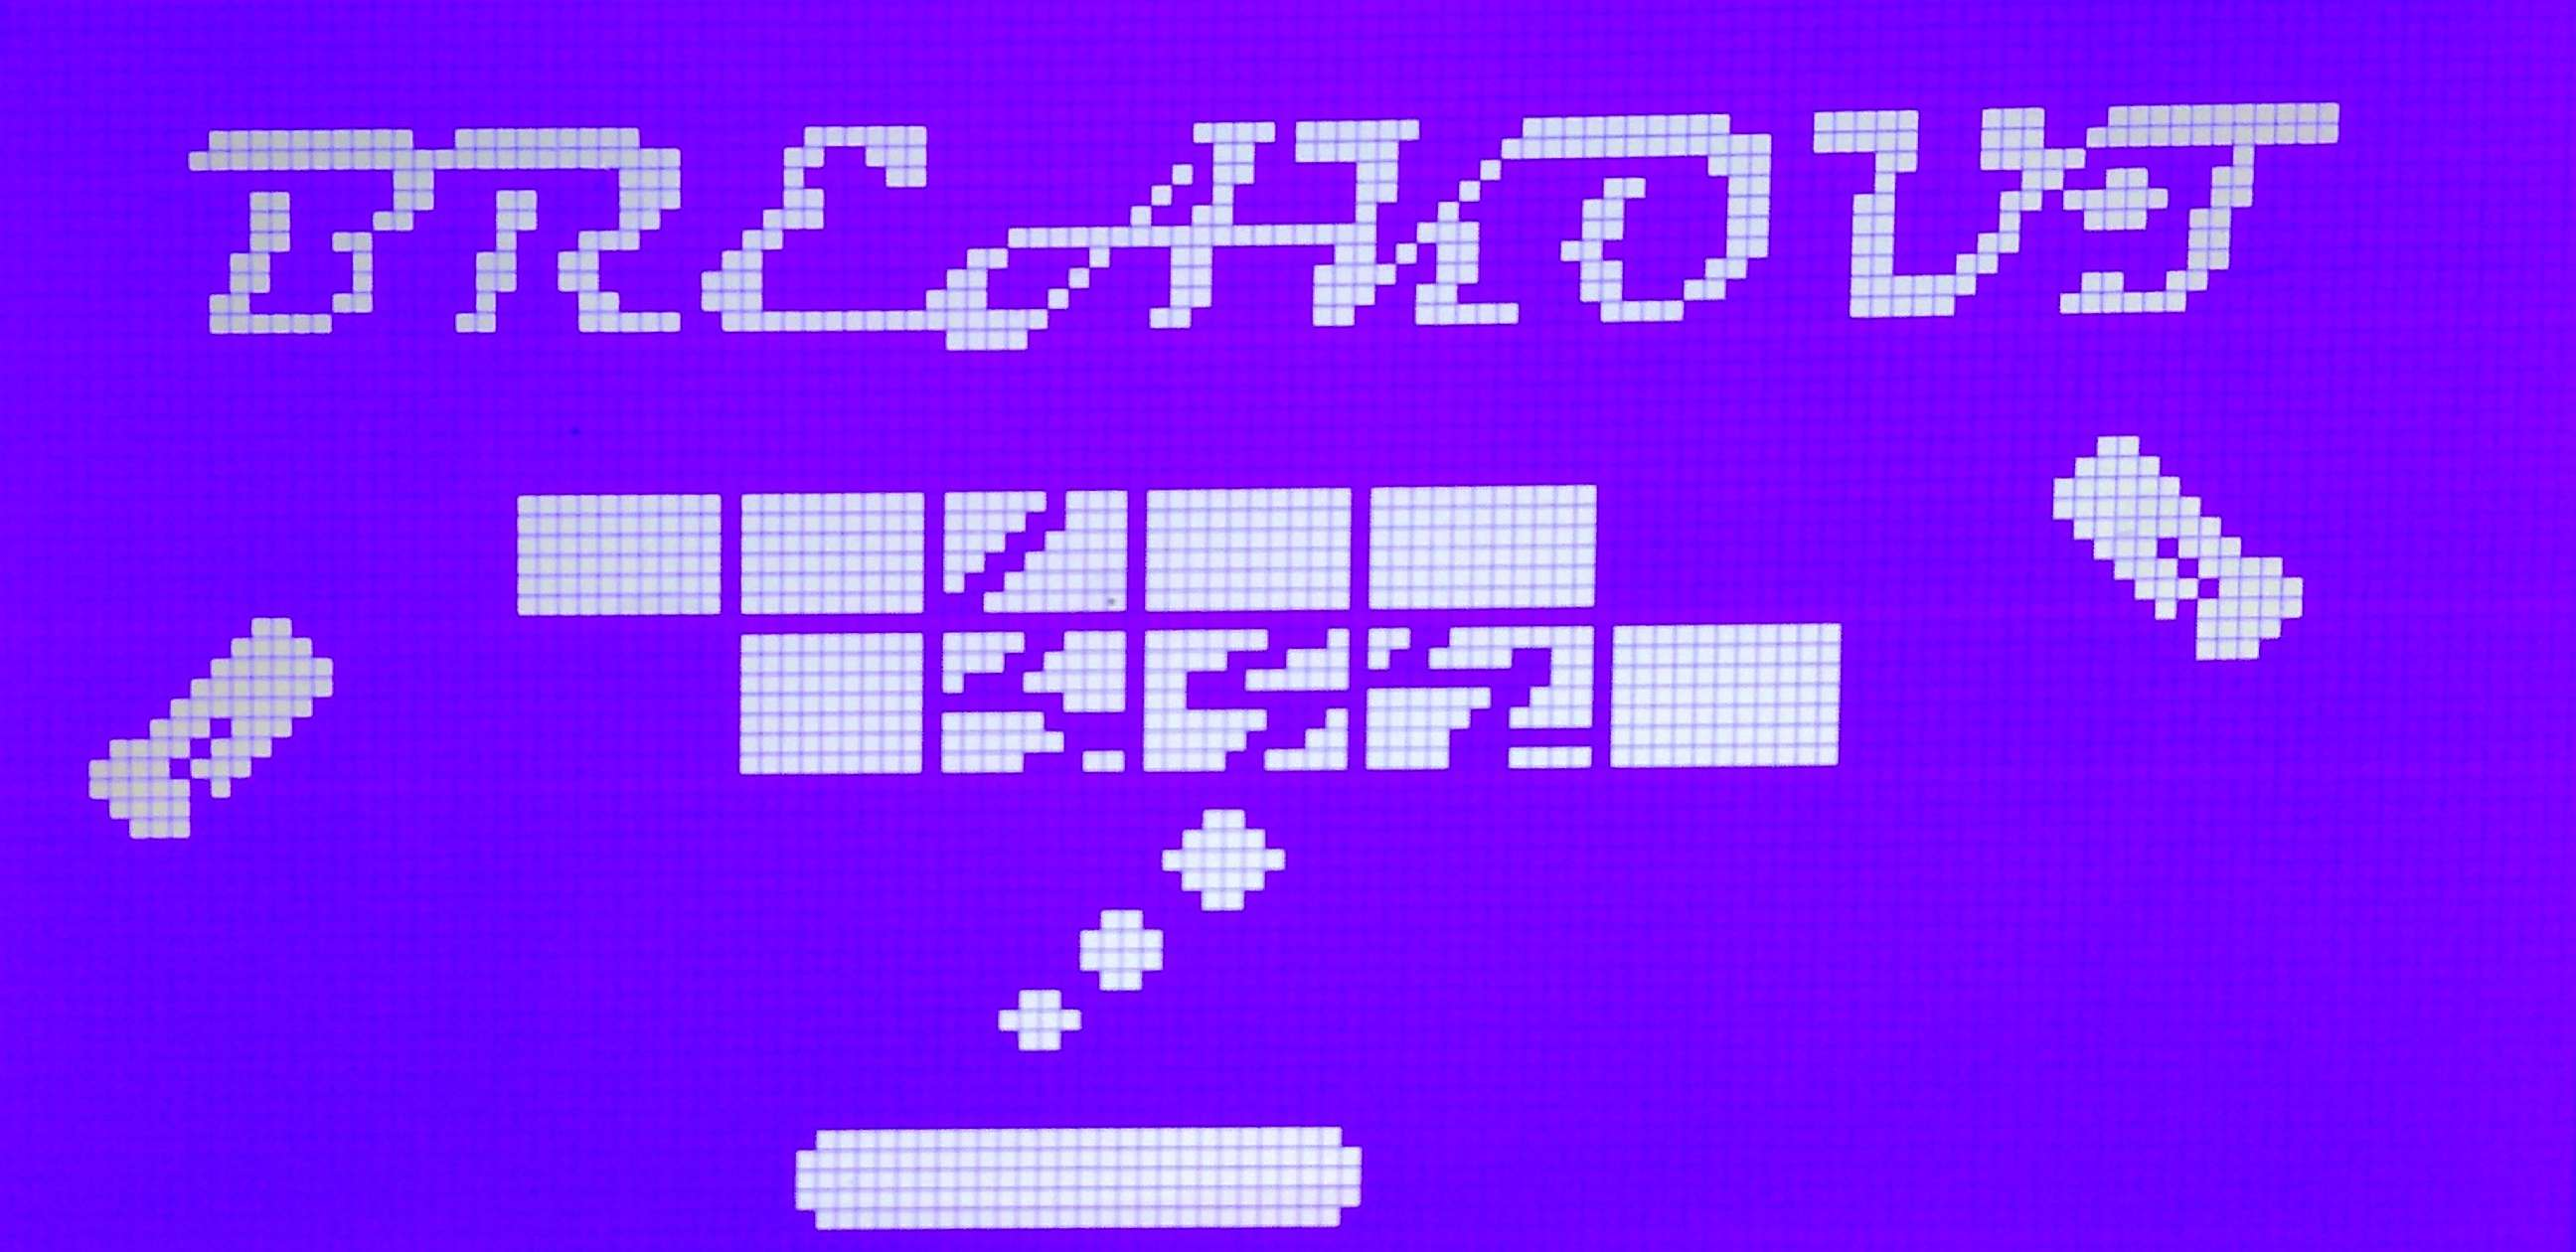
\includegraphics[width=10cm, height=5cm]{BreakoutImages/cutscene} \\
{\small Fig 5.3(a): Initial Cutscene, Music plays} \\
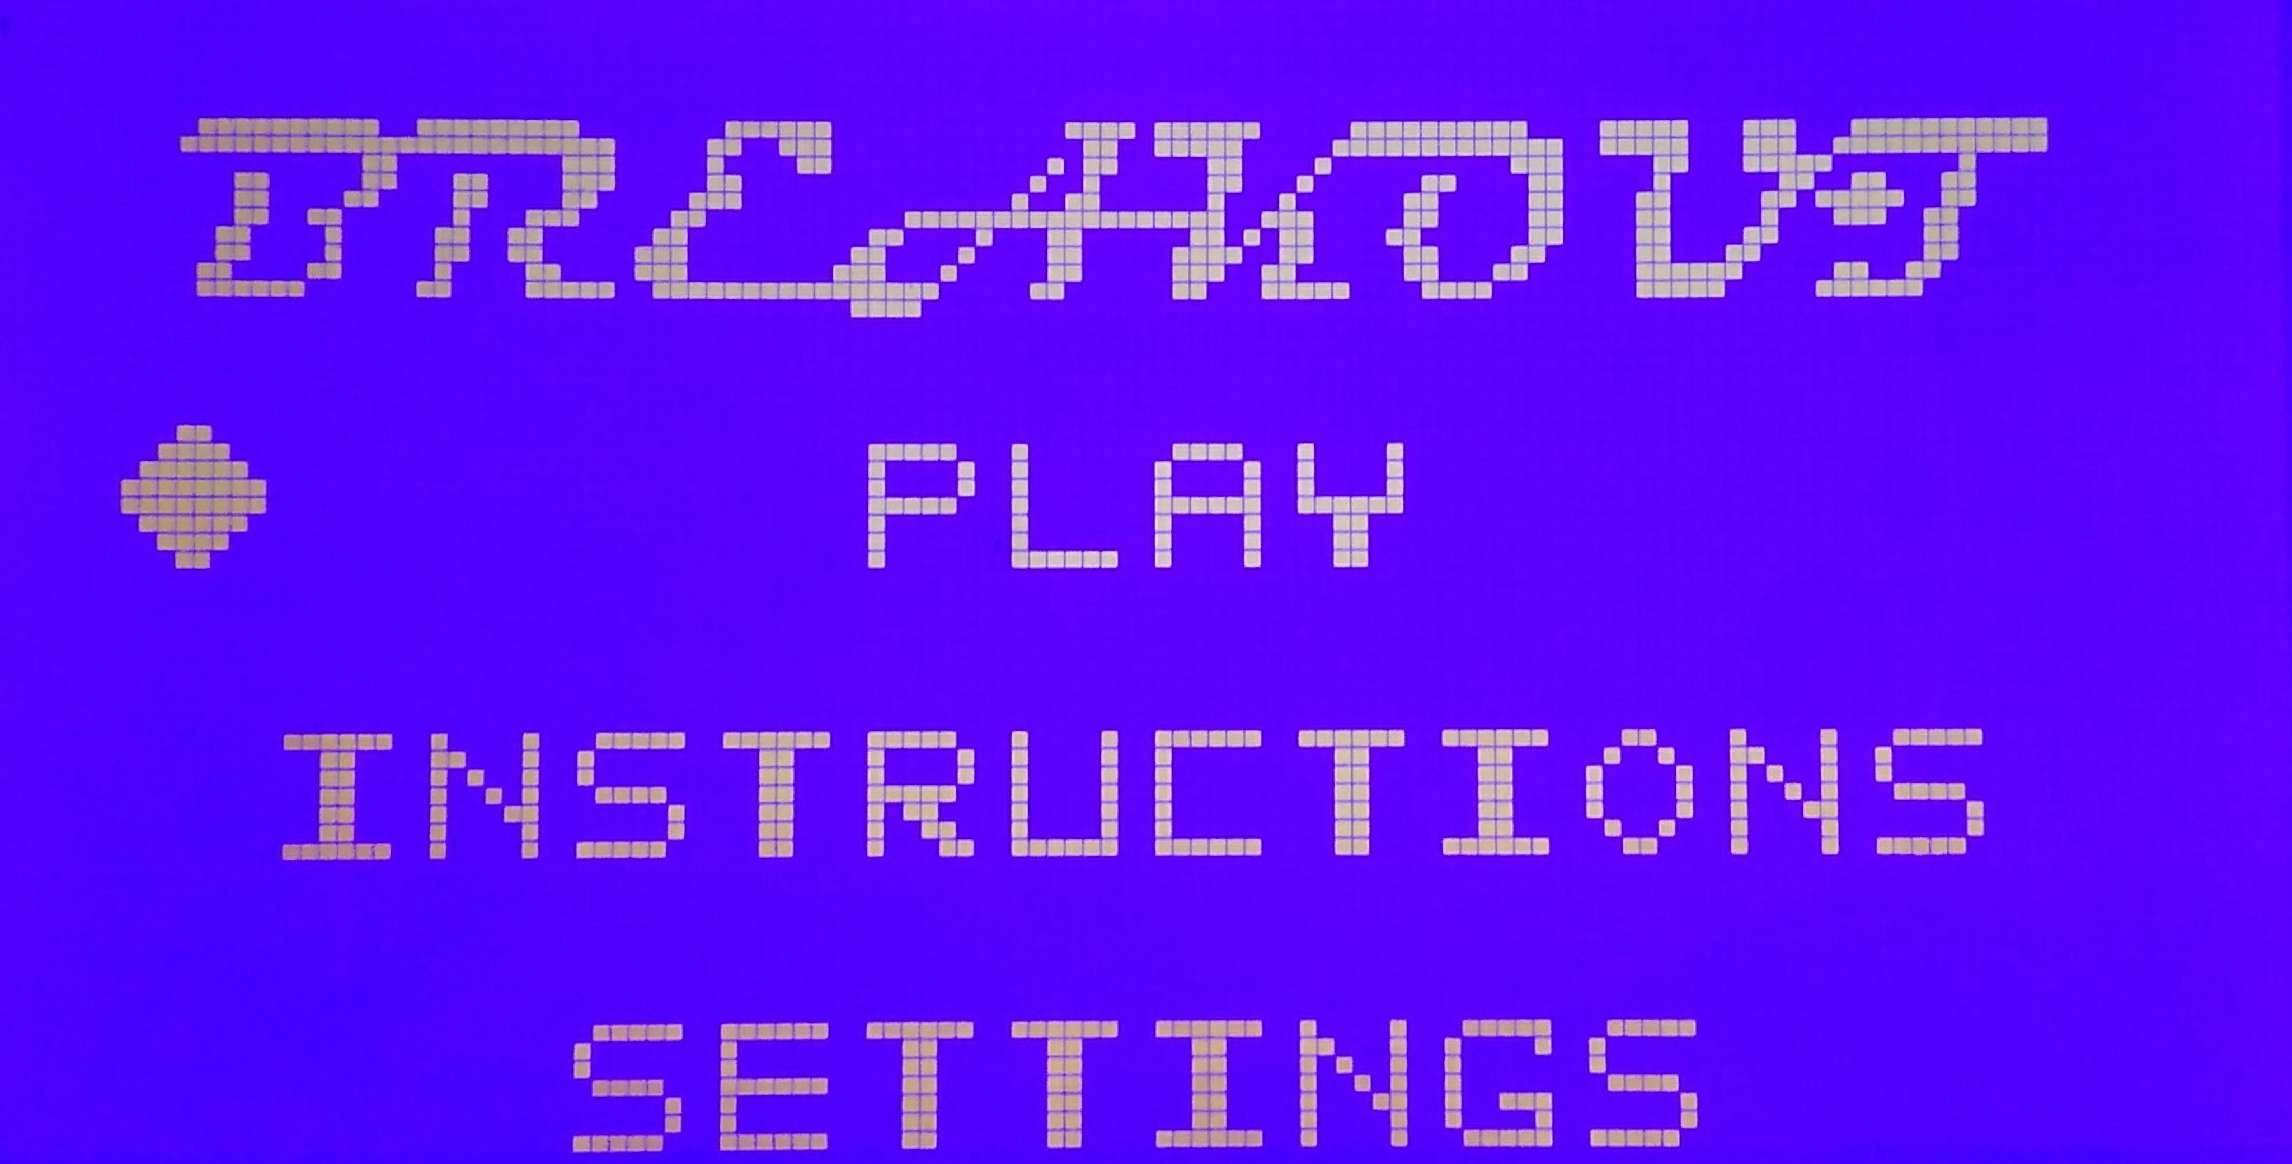
\includegraphics[width=10cm, height=5cm]{BreakoutImages/menuScreen} \\
{\small Fig 5.3(b): Menu Screen, with Cursor} \\
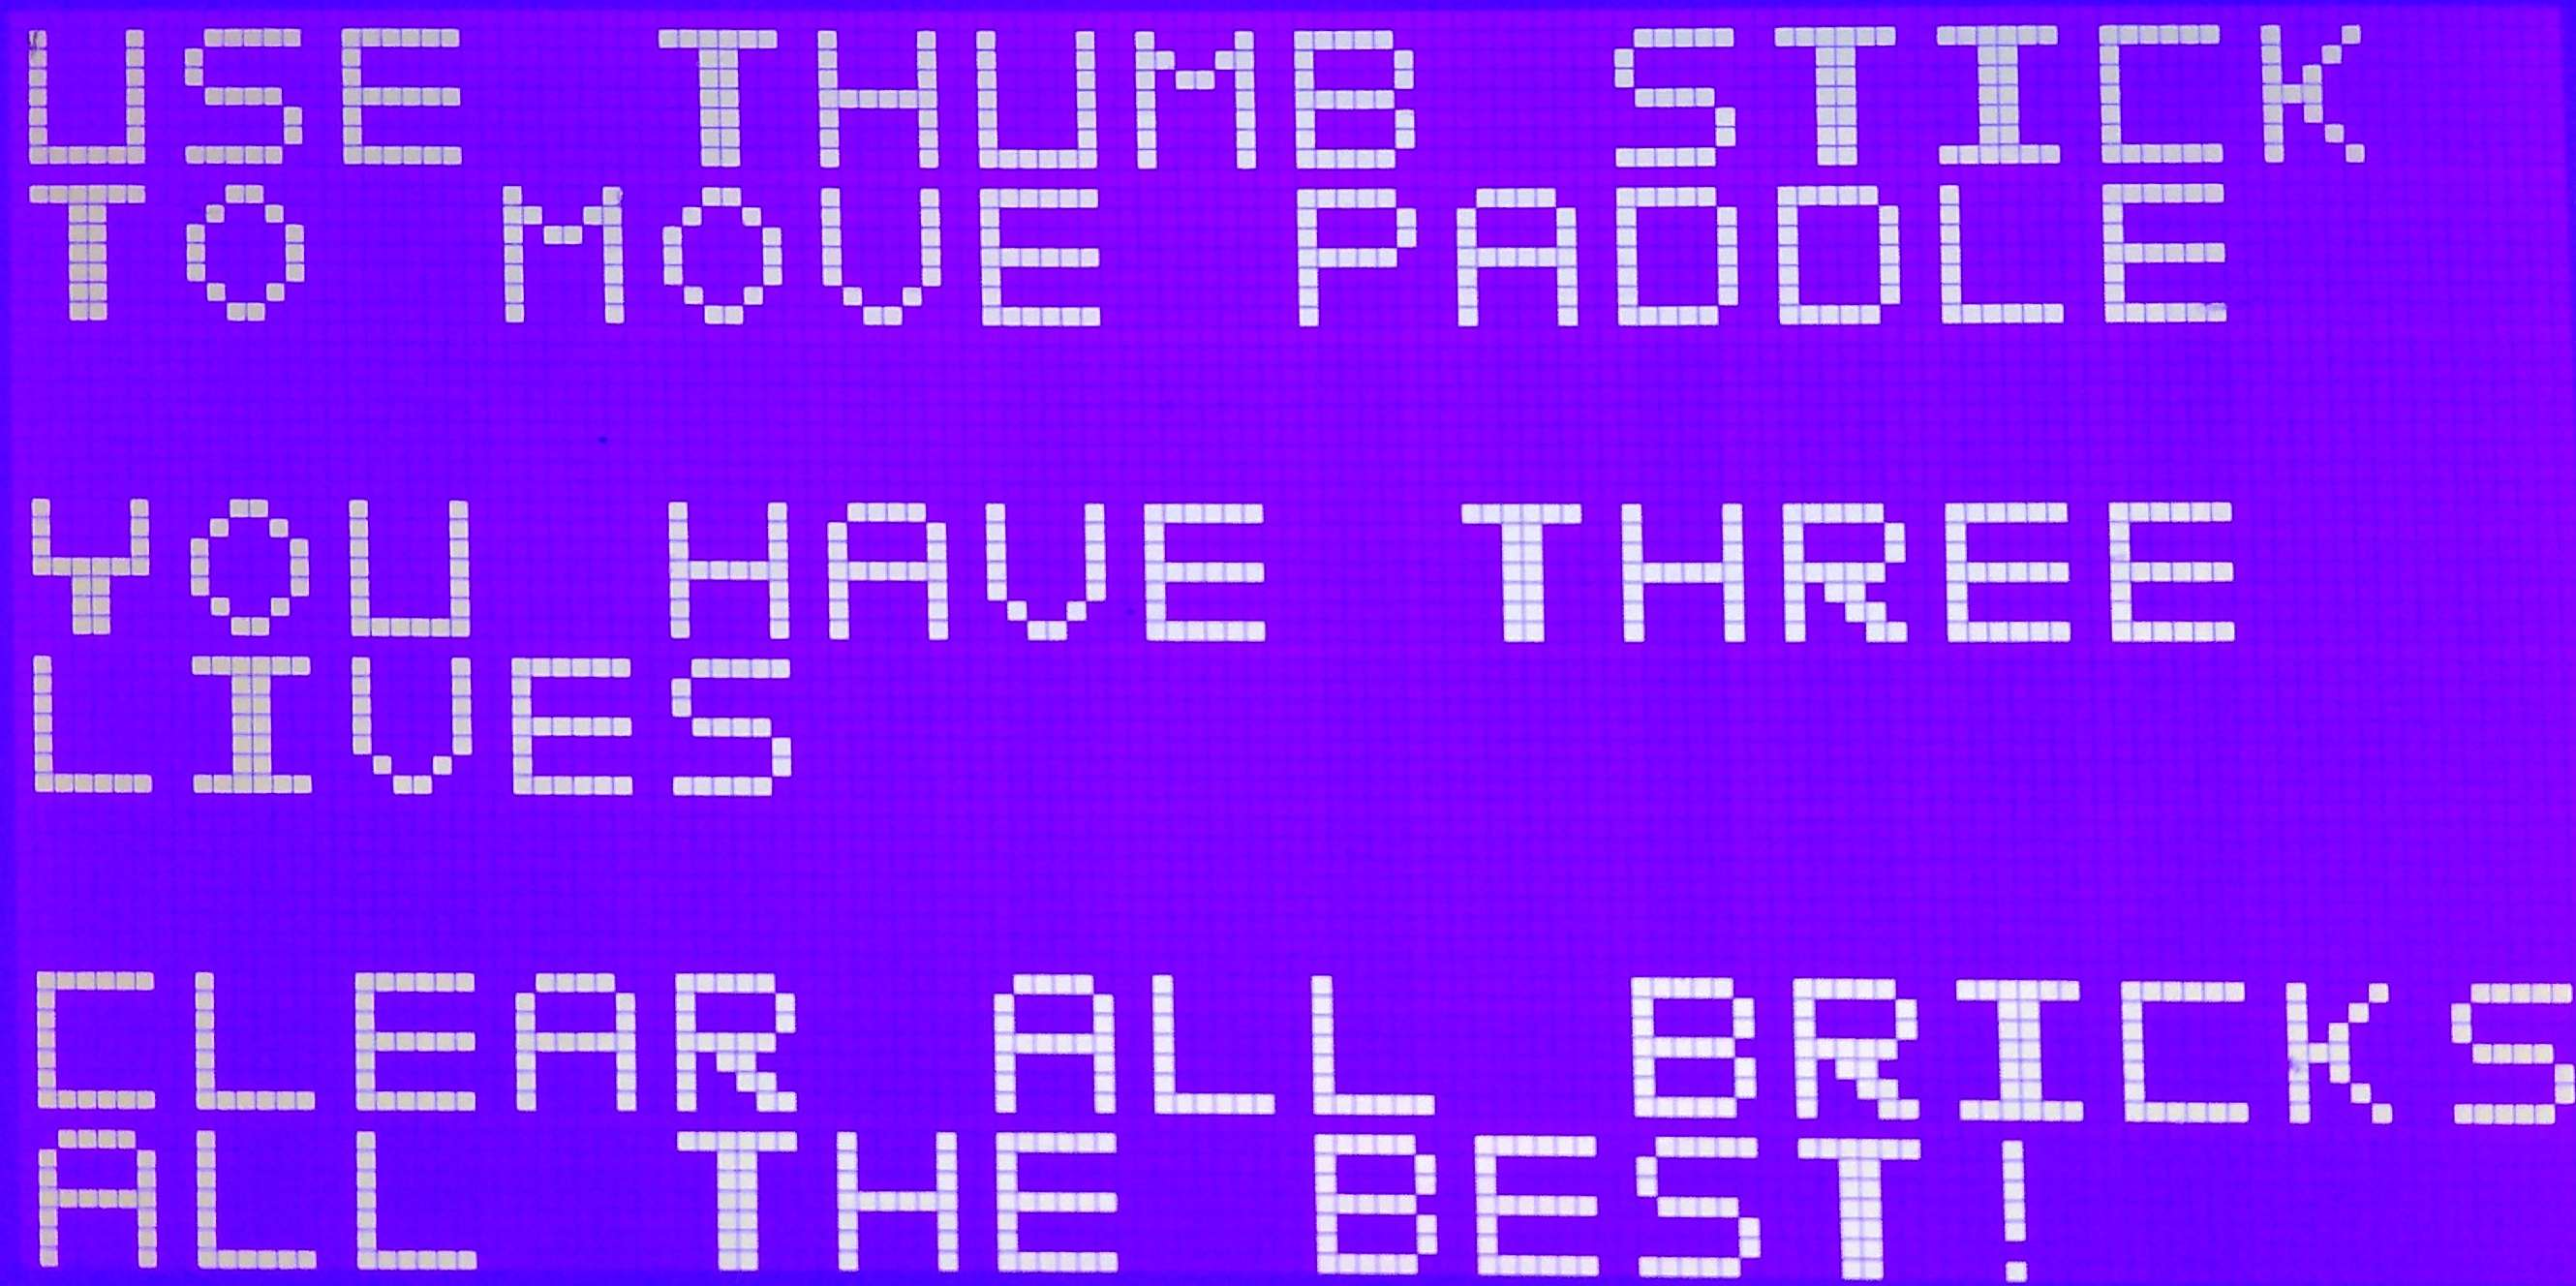
\includegraphics[width=10cm, height=5cm]{BreakoutImages/instructionsScreen} \\
{\small Fig 5.3(c): Instructions Screen} \\
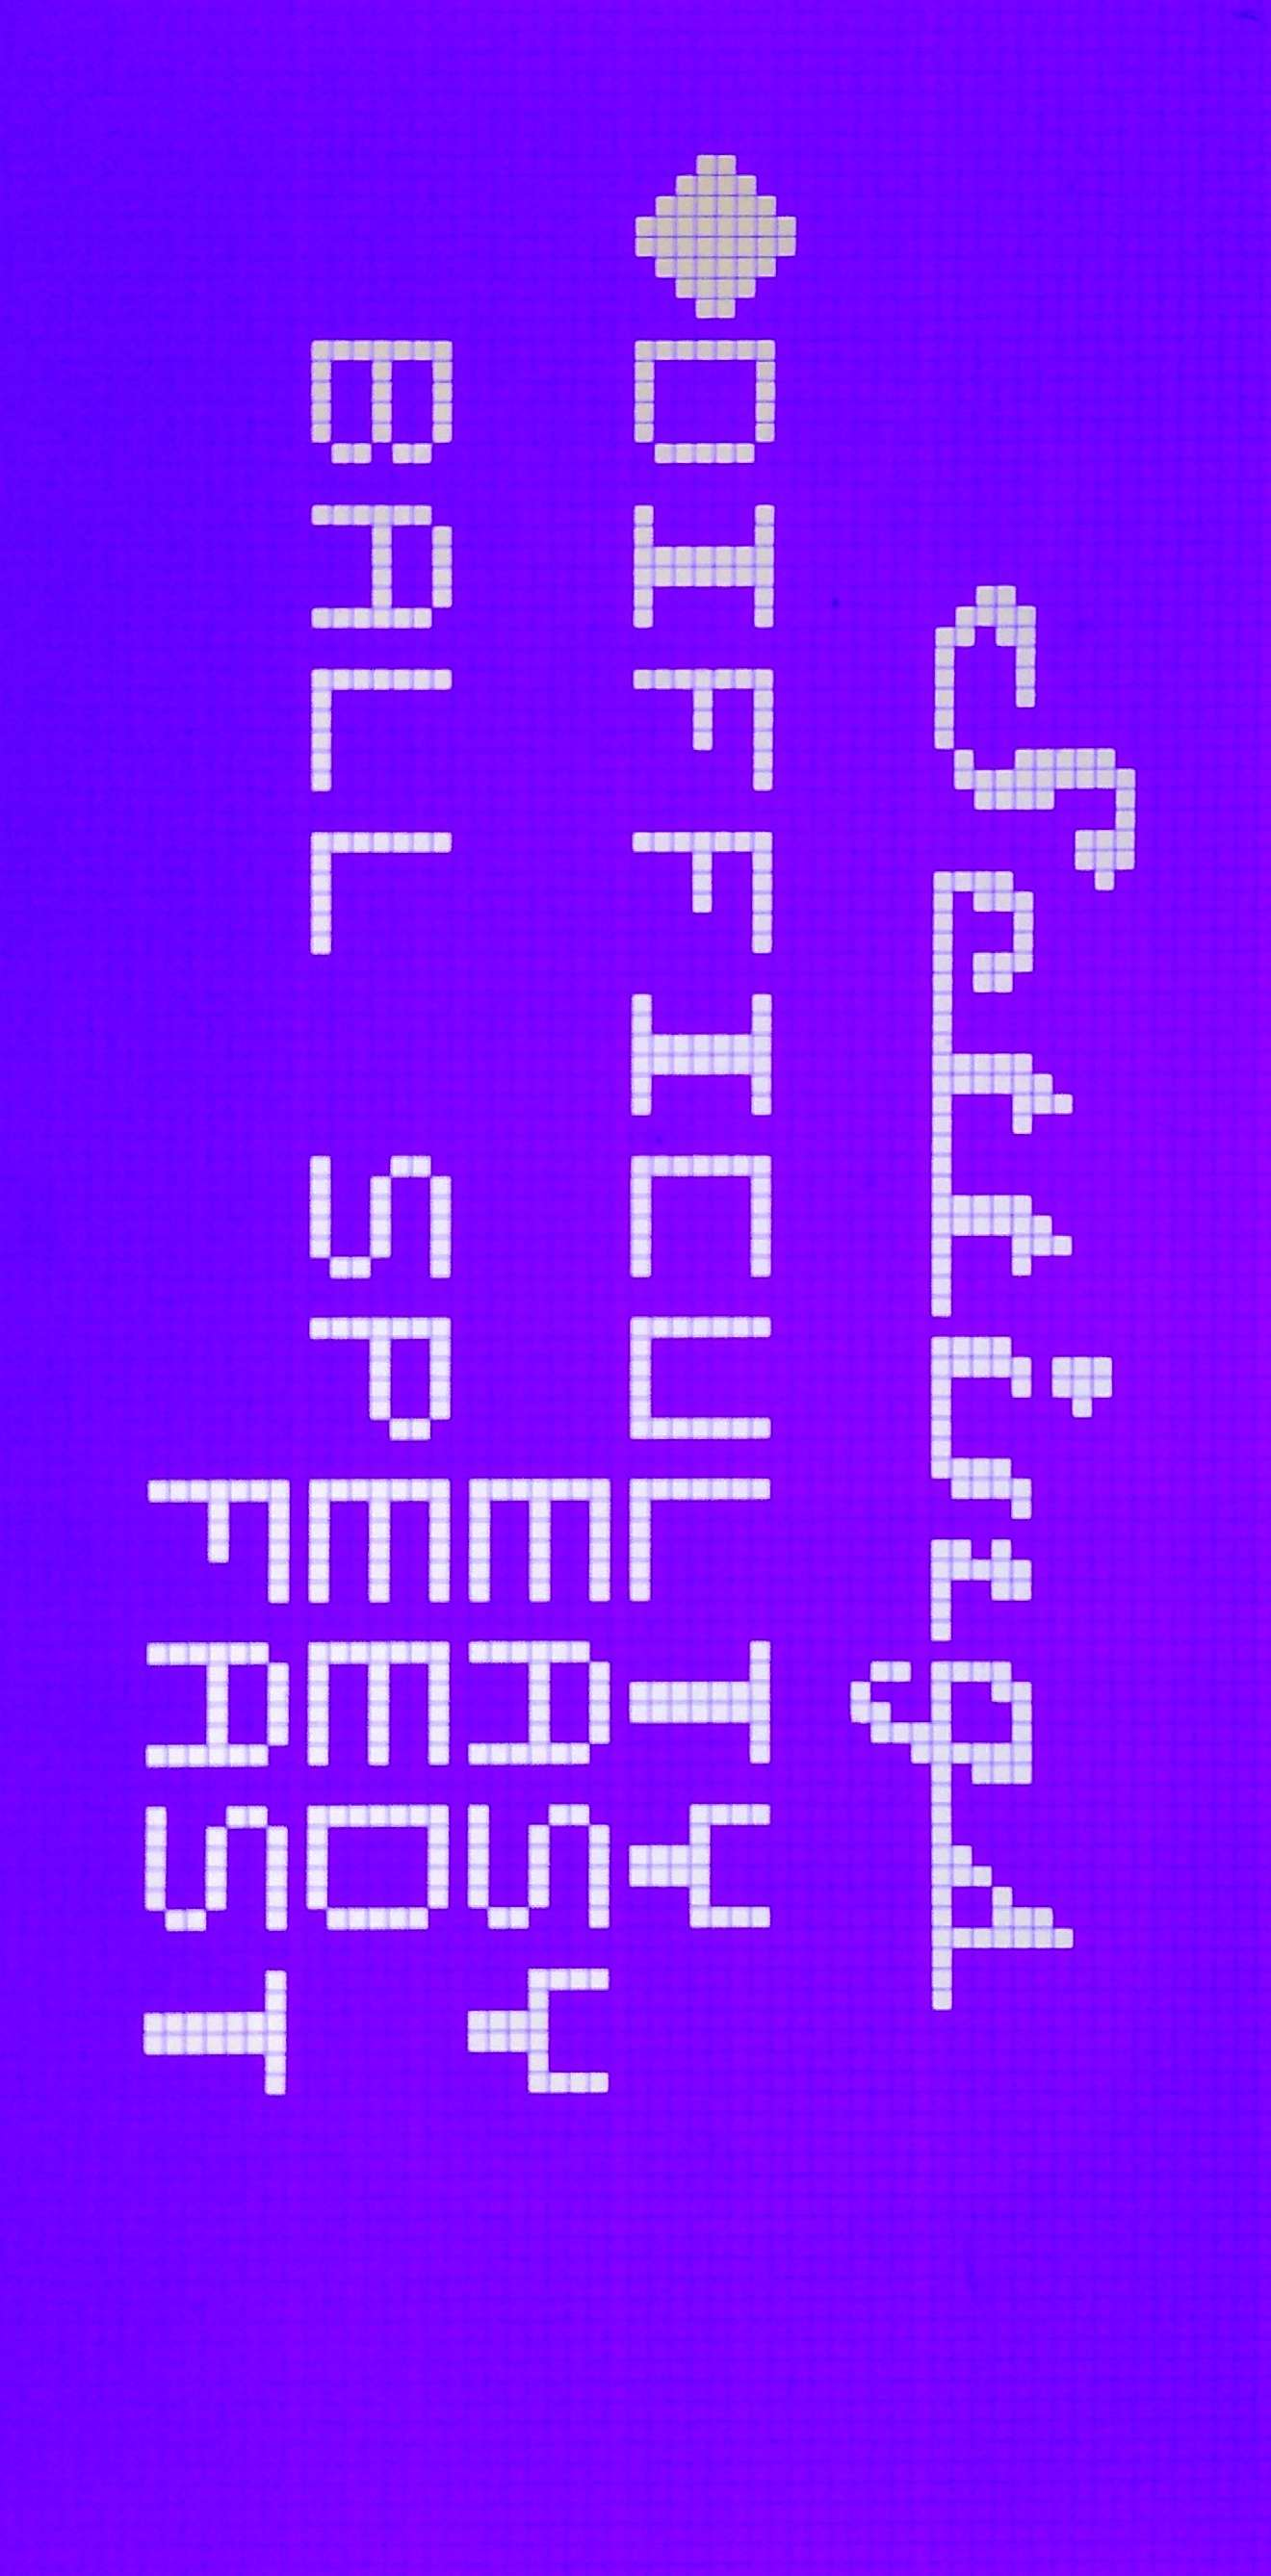
\includegraphics[width=5cm, height=10cm, angle = 90]{BreakoutImages/settingsScreen} \\
{\small Fig 5.3(d): Settings Screen} \\

\includegraphics[width=10cm, height=5cm]{BreakoutImages/livesDisplayScreen} \\
{\small Fig 5.3(e): Display Player Lives Screen} \\
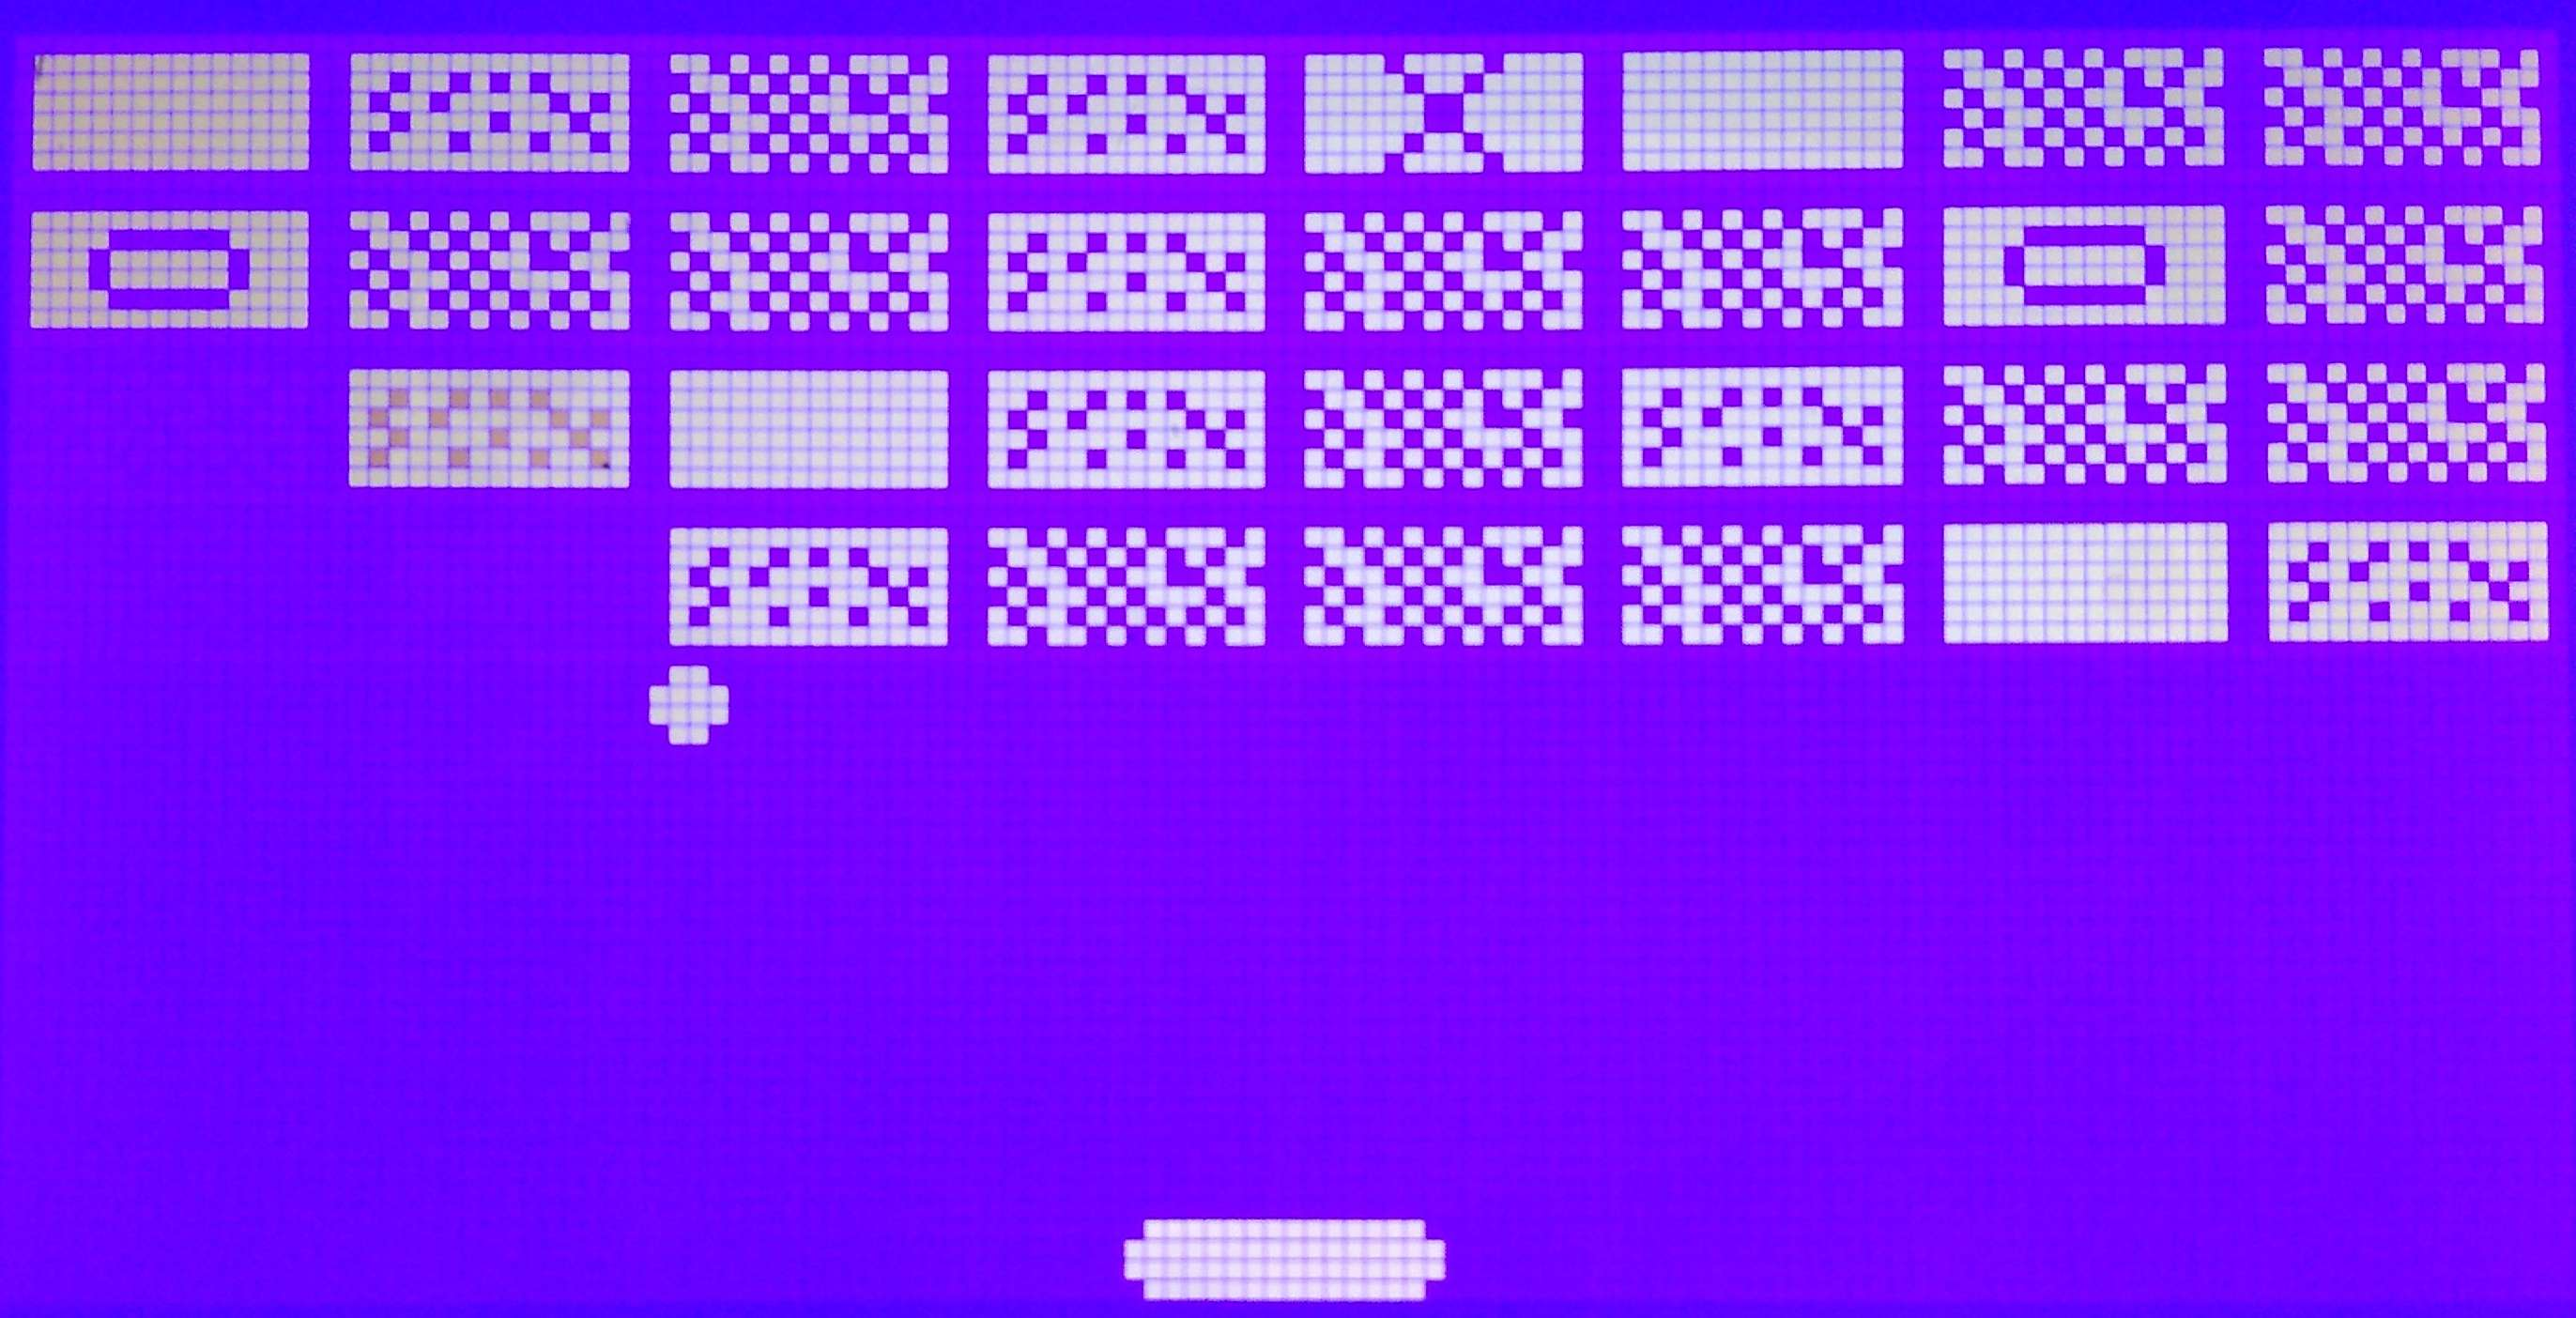
\includegraphics[width=10cm, height=5cm]{BreakoutImages/gameplayScreen} \\
{\small Fig 5.3(f): Gameplay Screen} \\
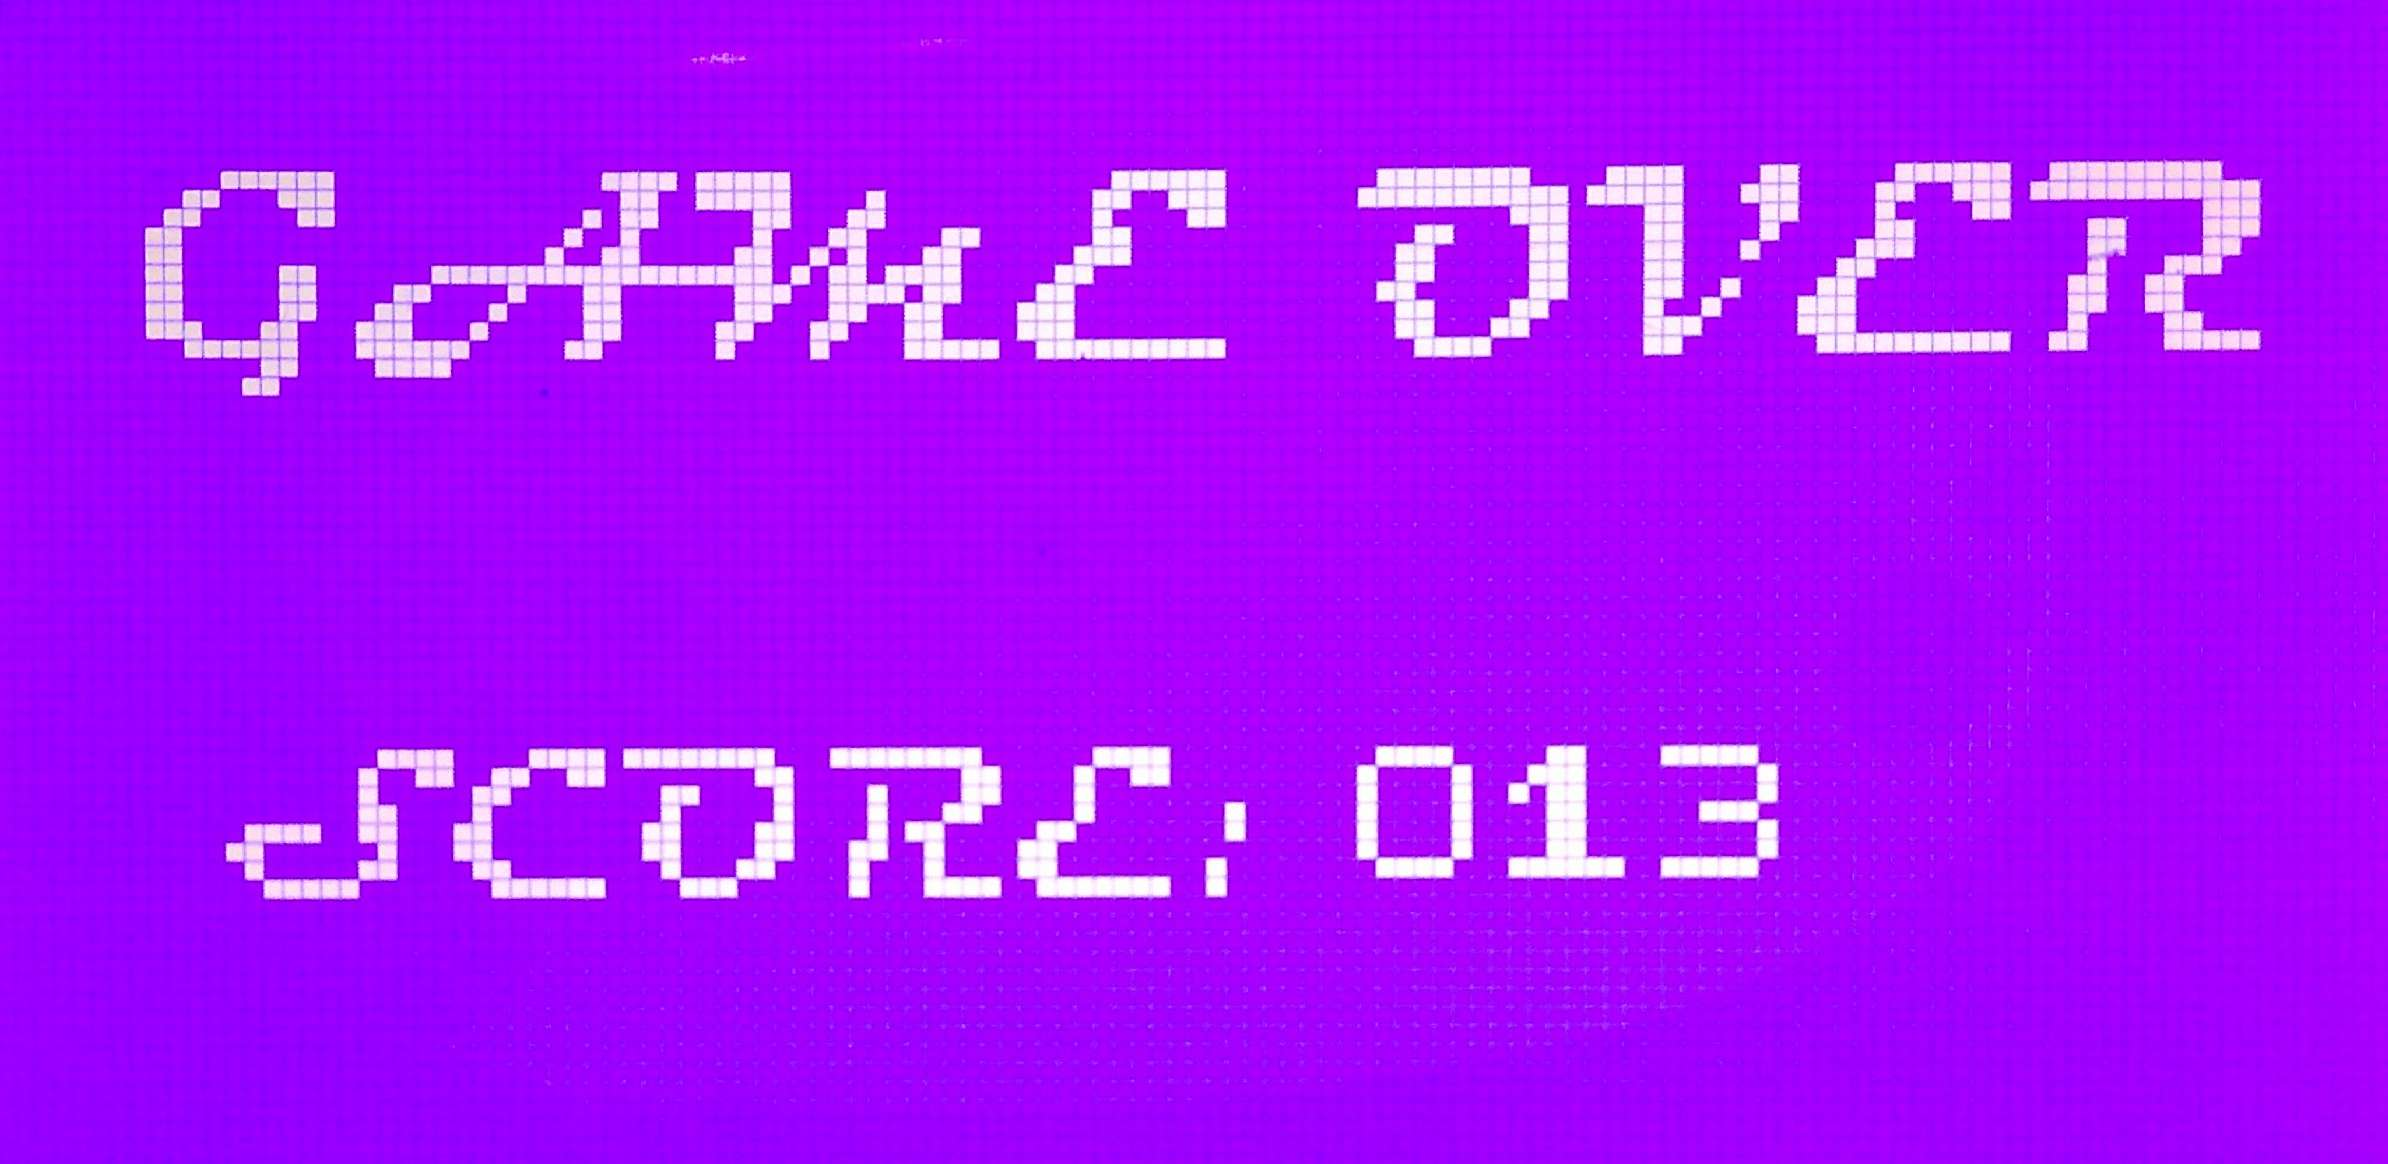
\includegraphics[width=10cm, height=5cm]{BreakoutImages/gameoverScreen} \\
{\small Fig 5.3(g): Game Over Screen} \\
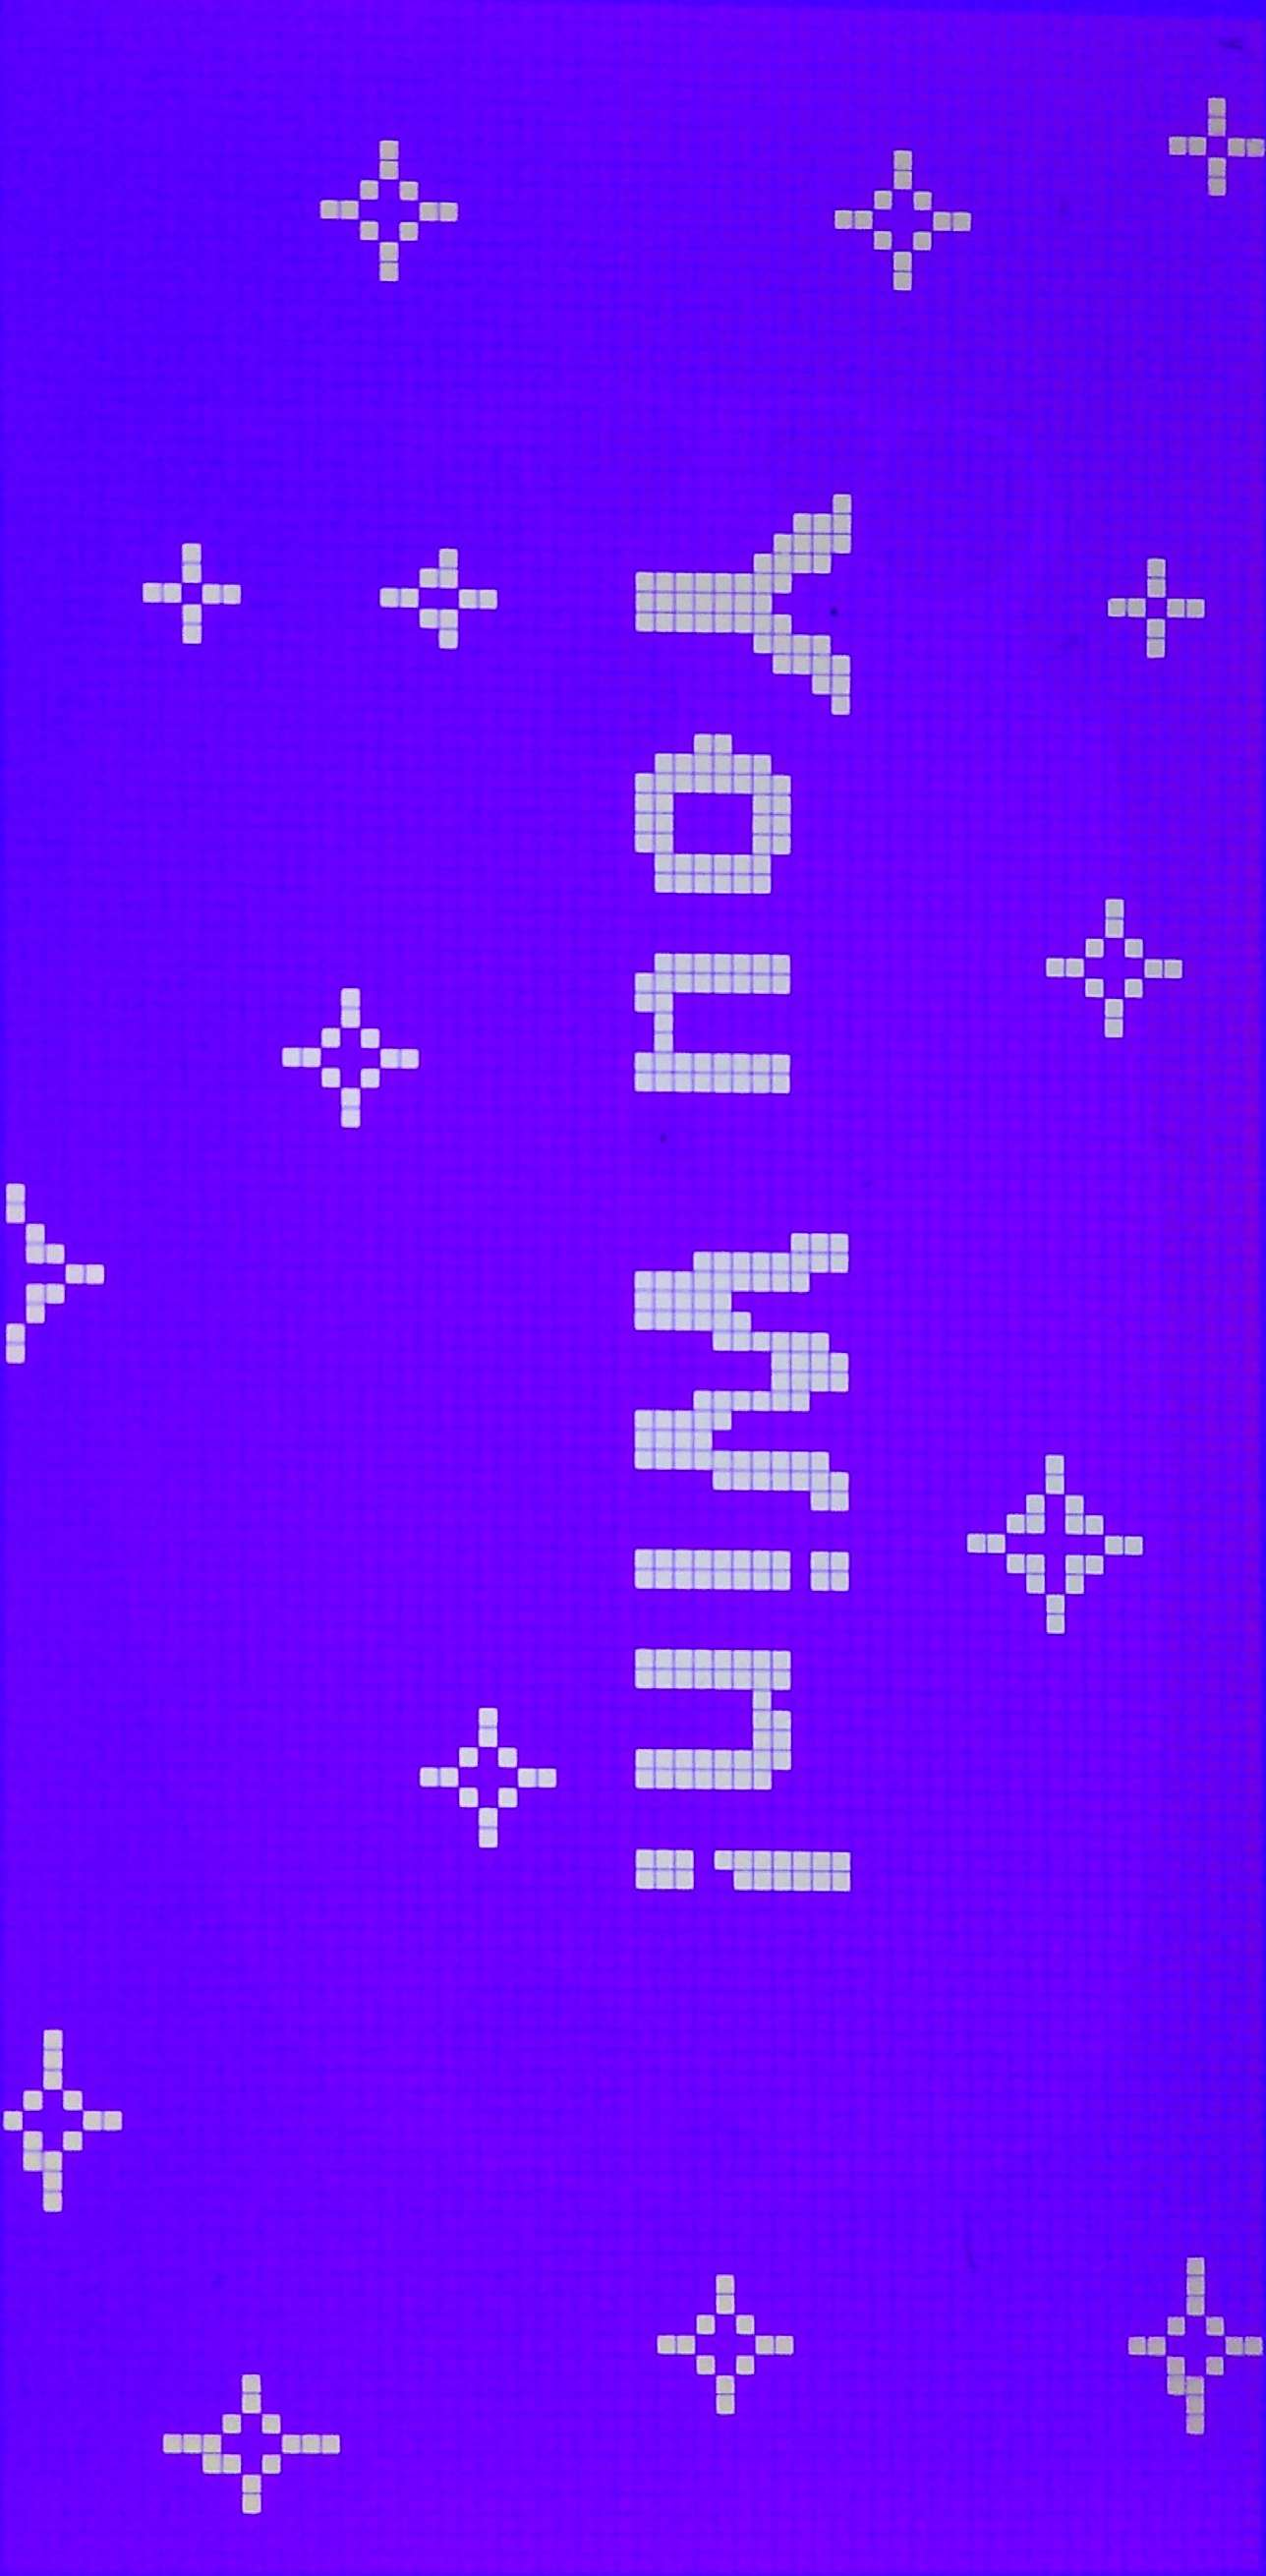
\includegraphics[width=5cm, height=10cm, angle  = 90]{BreakoutImages/victoryScreen} \\
{\small Fig 5.3(h): Victory Screen} \\
\end{center}

\chapter{Future Work}
\qquad We have provided a basement upon which much more complex games can be implemented using on-board hardware on the console, including tone libraries, glcd libraries, creating graphic, etc. Further innovation is possible in the following arenas:
\begin{enumerate}
\item Interfacing of a \textit{vibration} motor, which has been done, towards the end of our project, albeit with certain issues which can surely be improved upon. This provides better feedback during gameplay.
\item Interfacing of an \textit{angle sensor} like GY80 onto the board, which provides inclination values, which can be used for motion/tilt controlled gameplay.
\item \textit{Multiplayer gameplay} is also possible by connecting a Wi-Fi module or XBee to the board. Upon which data can be transmitted between one or more consoles while maintaining independent state machines on each console. Change of state transitions only need to be communicated.
\item The GLCD on the console can be replaced with a better resolution \textit{color LCD}, for better graphics and wider gameplay possibilities.
\item The Tiva C Launchpad can also be used in implementation of \textit{actuated systems}, including the Bomb Timer and Vending Machine examples.
\end{enumerate}

\chapter{Bug report and Challenges}
\section{Major Bugs Encountered}
\qquad There were several bugs encountered during the course of development, some of which are rectified, while others are not. They are as follows:
\begin{enumerate}
\item (\textit{Solved})The GLCD Display has an issue of \textit{one half of the screen not being initialized} at random instances(Does not happen all the time). In this case, a delay is added before and after the glcd\_cmd(0x3F) command in glcd\_init() in the GLCD library to remove the error.
\item (\textit{Solved}) If certain game objects reference portions of GLCD which are out of bounds(like row < 0 or row > 7 or column < 0 or column > 128), \textit{unpredictable behaviour} occurs on screen. So ensure that the row and column variables remain always within limits. Encountered using paddle implementation.
\item (\textit{Unsolved})The block wall is \textit{not randomized} in spite of using the randomizer(rand() in C), because, since the randomizer is executed in C by the compiler, the \textit{numbers are pre-generated} and stored in the hex file which is dumped onto the board. And hence, the blocks remain unrandomized till a fresh program is loaded onto the board. A proposed solution is to use a timer to make the randomizer generate a seed number based on time taken by the user to press play. 
\item (\textit{Unsolved})The \textit{Buzzer has distinct output frequencies at different points of time}, and some of the tones sound weird at random times. But this is restricted to hardware capabilities of the buzzer and is not an error in code. 
\item (\textit{Unsolved})The \textit{vibration motor is not responsive} to shortlived ON and OFF actions in code. And only works at certain random instances. Proposed solution is to use a better motor.
\item (\textit{Unsolved})The \textit{moving ball on screen remains uncleared} at certain instances on screen, even after an explicit clear command. Adding of delay during ball clear is of little use. And the problem persists.
\item (\textit{Unsolved}) When strings are displayed using the font library, certain \textit{characters appear at random rows} inspite of explicit specification of a certain row and cursor position. Reasons unknown. 
\end{enumerate}
\section{Challenges Faced}
\qquad During the course of the project, there were several challenges faced, as follows:
\begin{enumerate}
\item The learning challenge of familiarising with the Tiva C Board and its peripherals. Of the labs, especially PWM was particularly challenging.
\item Understanding statecharts and its code implementation was another challenge. Required rethinking of how we approach the problem. Extensive use of switchcase was required.
\item The absence of software to create graphic for GLCD directly of the required size. This required use of the font creator and its tideous export process to create certain graphic and the larger sized font.
\item The creation of the tones library.
\item Design of the game and creation of the statechart for the game. Debugging of several encountered bugs.
\end{enumerate}
\section{Failures}
\begin{enumerate}
\item The earlier intention to provide a Quantum Framework library for development on the Tiva C could not be realised because of the complex nature of the QPC Platform.
\item The State Table implementation of the Statecharts also proved an unassailable task because of little familiarisation with C structures.
\end{enumerate}
\begin{thebibliography}{li}
\bibitem{datasheet}
{\em \href{http://www.ti.com/lit/ds/spms376e/spms376e.pdf}{TM4C123GH6PM Data Sheet}}
\bibitem{tivactutorial}
{\em \href{http://software-dl.ti.com/trainingTTO/trainingTTO_public_sw/GSW-TM4C123G-LaunchPad/TM4C123G_LaunchPad_Workshop_Workbook.pdf}{Tiva C Workbook}}
\bibitem{tirtostutorial}
{\em \href{http://www.ti.com/lit/ug/spruhd4m/spruhd4m.pdf}{TI-RTOS 2.20 User's Guide}}
\bibitem{statechart}
David Harel and A Pneuli,
{\em Statecharts: A Visual Formalism for Complex Systems},
1987.
\bibitem{quantumframework}
Miro Samek,
{\em Practical UML Statecharts in C/C++,ISBN: 978-0-7506-8706-5},
2009.
\end{thebibliography}

\end{document}